\section{Introduction}

Food waste is a growing global concern. Restaurants, households, and event organizers often discard large amounts of leftover food, while many individuals struggle to obtain adequate meals. The lack of coordination between food donors and charitable organizations leads to unnecessary food wastage.

The Food Donation Management System is designed to address this problem by providing a centralized platform where donors can list surplus food items and NGOs can request them for distribution. The system simplifies communication and coordination between donors and organizations.

Through this web application, donors can easily register and contribute leftover food, NGOs can browse available donations and submit requests, and administrators can monitor and approve requests to ensure transparency and accountability.

This system aims to promote social welfare while reducing food waste through the use of modern web technologies.



\vspace{30pt}
\section{Objectives}

The main objectives of the project are:

\begin{enumerate}
\item To reduce food wastage by connecting food donors with NGOs.
\item To create a centralized digital platform for managing food donations.
\item To allow donors to easily list available food donations.
\item To enable NGOs to request food donations efficiently.
\item To provide administrative control for approving and managing donation requests.
\item To improve the efficiency and transparency of food distribution.
\item To support humanitarian efforts through technology.

\end{enumerate}

\vspace{20pt}
\section{Literature Review / Background Study}

Food waste and hunger are two interconnected global challenges that affect millions of people worldwide. According to the Food and Agriculture Organization (FAO), approximately one-third of the food produced globally for human consumption is lost or wasted each year, which equals nearly 1.3 billion tons of food annually \cite{gustavsson2011global}. At the same time, the United Nations reports that hundreds of millions of people still suffer from hunger and food insecurity. This imbalance between food surplus and food scarcity highlights the urgent need for systems that can efficiently redistribute excess food to people in need.

Researchers and international organizations have increasingly emphasized the role of technology in addressing food waste and improving food distribution. Digital platforms and web-based systems can connect food donors, such as restaurants and households, with charitable organizations responsible for distributing food to vulnerable populations. These systems improve communication and coordination between donors and NGOs, allowing surplus food to be identified and distributed more efficiently before it becomes waste \cite{forbes2021food}.

Traditional food donation processes often rely on informal communication methods such as phone calls, personal contacts, or social media posts. These approaches are often inefficient and lack transparency, making it difficult to track donations or coordinate timely distribution. Studies indicate that the absence of centralized digital platforms is one of the major barriers to effective food redistribution. Implementing structured information systems can significantly improve the management of food donations and reduce food wastage \cite{michelini2018understanding}.

Several food-sharing initiatives and digital platforms have been developed globally to address these issues. These platforms allow individuals, restaurants, and businesses to donate surplus food through online systems that coordinate requests and distribution. Research has shown that such platforms can reduce food waste while strengthening community engagement and social responsibility \cite{papargyropoulou2014food}. In addition, data management within these systems enables better monitoring of donations, improved resource allocation, and more efficient coordination among participating organizations \cite{atukunda2021unlocking}.

Food redistribution initiatives are closely related to the United Nations Sustainable Development Goals (SDGs). In particular, SDG-2: Zero Hunger aims to end hunger, achieve food security, and improve nutrition for all people by 2030. One of the strategies to support this goal is improving access to food resources and strengthening food distribution networks \cite{lee2016transforming}. By facilitating the transfer of surplus food to charitable organizations, digital food donation platforms can contribute to reducing hunger and improving food availability for vulnerable populations.
Furthermore, SDG-12: Responsible Consumption and Production emphasizes reducing food waste across production and consumption systems. Target 12.3 specifically aims to halve global food waste at the retail and consumer levels by 2030 \cite{flanagan2019reducing}. Technology-driven food donation systems can play an important role in achieving this objective by enabling efficient food redistribution and promoting responsible consumption practices.

Based on these research findings, the Food Donation Management System proposed in this project aims to provide a structured web-based platform that connects food donors with NGOs responsible for distributing food to people in need. By leveraging digital technology and centralized data management, the system seeks to reduce food waste, improve donation coordination, and contribute to global efforts to achieve Zero Hunger and Responsible Consumption.



\vspace{40pt}
\section{Survey Questionnaires}

\begin{enumerate}
\item A digital platform for food donation and distribution would make it easier for people to donate surplus food.
\item An online system could help connect food donors with organizations that distribute food to the needy.
\item Technology can play an important role in reducing food wastage in society.
\item People would be more willing to donate food if a convenient online system were available.
\item A food donation system should provide clear information about where and when food can be collected.
\item A food donation system should display the current status of food donations (for example, pending, collected, or delivered).
\item A food donation system should have a user-friendly dashboard for different types of users.
\item A food donation platform should ensure the security and privacy of user information.
\item A food donation system should allow users to view their past donation or request history.
\item Search and filtering options would be useful for finding relevant food donations.
\item Please share any additional comments, suggestions, or opinions you have about our 'Food Donation and Distribution System'.

\end{enumerate}




\vspace{30pt}

\section{Response Summary}

\begin{figure}[H]
\centering
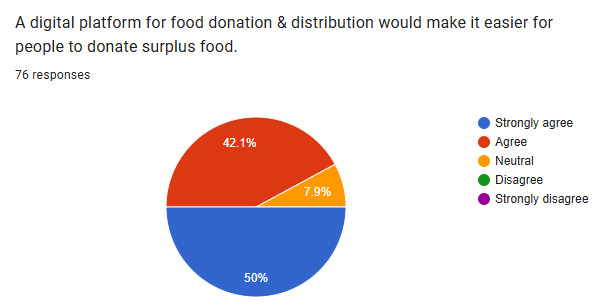
\includegraphics[width=0.75\textwidth]{Images/1.jpg}

Survey Response for Q1
\end{figure}



\begin{figure}[H]
\centering
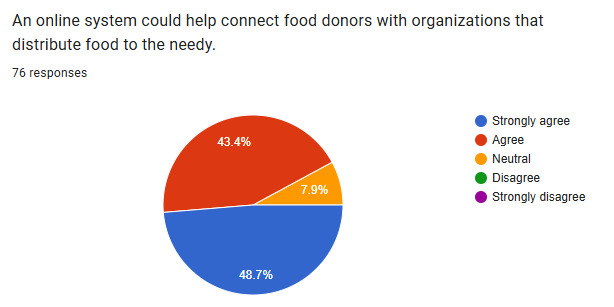
\includegraphics[width=0.75\textwidth]{Images/2.jpg}

Survey Response for Q2
\end{figure}


\begin{figure}[H]
\centering
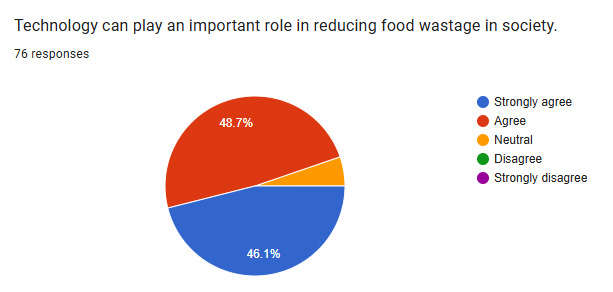
\includegraphics[width=0.75\textwidth]{Images/3.jpg}

Survey Response for Q3
\end{figure}




\begin{figure}[H]
\centering
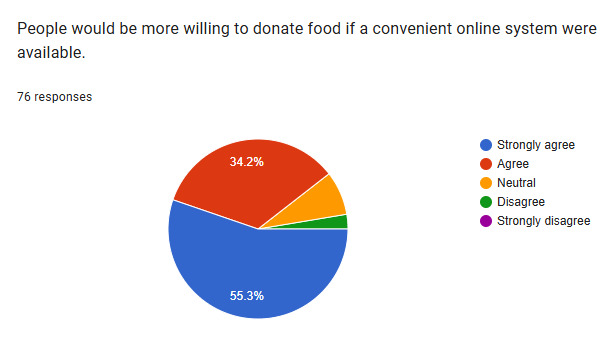
\includegraphics[width=0.75\textwidth]{Images/4.jpg}

Survey Response for Q4
\end{figure}


 

\begin{figure}[H]
\centering
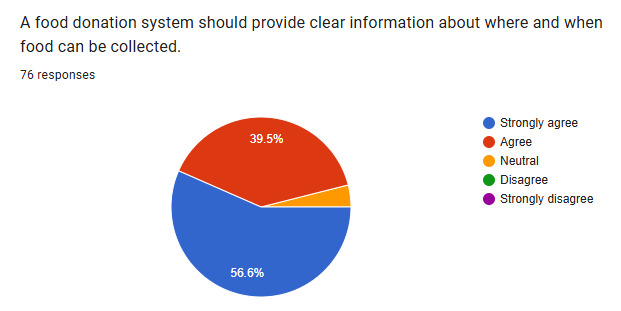
\includegraphics[width=0.75\textwidth]{Images/5.jpg}

Survey Response for Q5
\end{figure}



  
\begin{figure}[H]
\centering
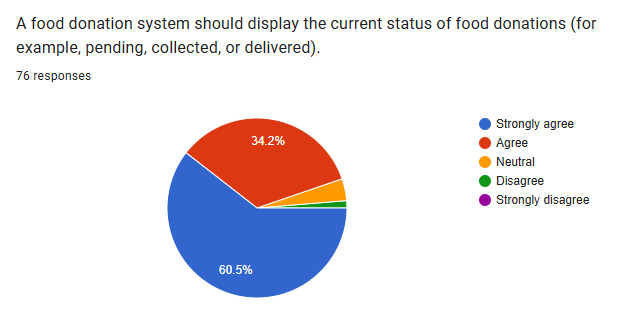
\includegraphics[width=0.75\textwidth]{Images/6.jpg}

Survey Response for Q6
\end{figure}




\begin{figure}[H]
\centering
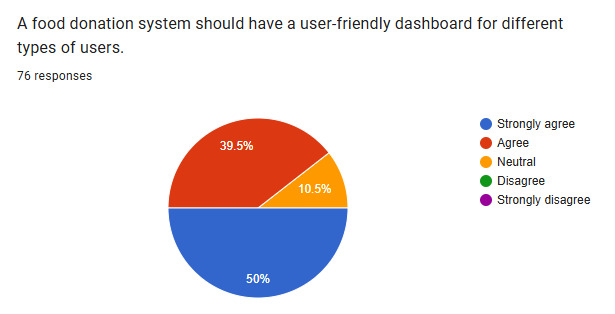
\includegraphics[width=0.75\textwidth]{Images/7.jpg}

Survey Response for Q7
\end{figure}




\begin{figure}[H]
\centering
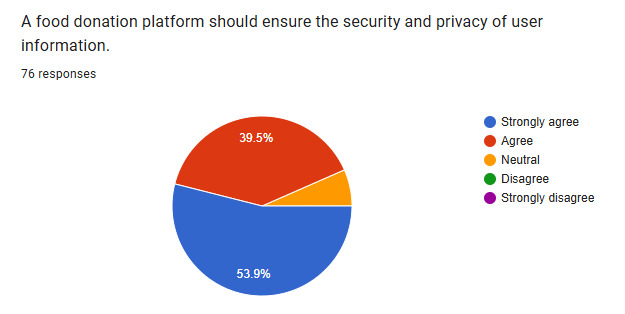
\includegraphics[width=0.75\textwidth]{Images/8.jpg}

Survey Response for Q8
\end{figure}




\begin{figure}[H]
\centering
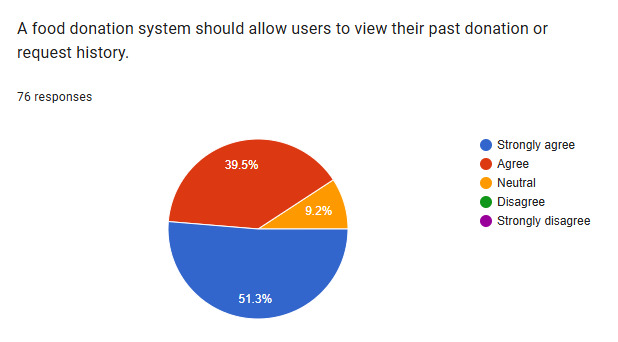
\includegraphics[width=0.75\textwidth]{Images/9.jpg}

Survey Response for Q9
\end{figure}




\begin{figure}[H]
\centering
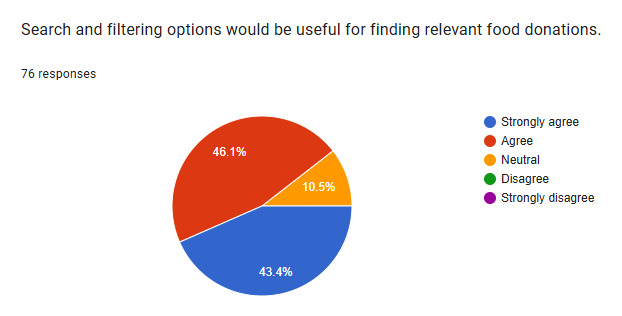
\includegraphics[width=0.75\textwidth]{Images/10.jpg}

Survey Response for Q10
\end{figure}
\FloatBarrier



\vspace{140pt}
\section{Problem and Solution Description}

\textbf{Problem:} Large quantities of food are wasted daily while many people remain hungry. There is often no structured system to connect food donors with organizations that distribute food to the needy.
Key issues include:
\begin{itemize}
\item Lack of coordination between donors and NGOs
\item Inefficient manual communication
\item Food spoilage due to delays
\item No centralized tracking system
\end{itemize}

\vspace{10pt}
\textbf{Solution:} The proposed solution is a web-based Food Donation Management System that:
\begin{itemize}
\item Allows donors to add food donation information.
\item Enables NGOs to browse and request available donations.
\item Allows administrators to approve or reject requests.
\item Maintains a database for managing donations and requests.

\end{itemize}
This solution improves communication, reduces food waste, and promotes social responsibility.






\vspace{30pt}
\section{Addressing UN Sustainable Development Goals}

This project supports the following United Nations Sustainable Development Goals (SDGs):

 \vspace{5pt}
\textbf{SDG 2 – Zero Hunger}
 The system helps distribute surplus food to people in need through NGOs.
 \vspace{10pt}
 
\textbf{SDG 12 – Responsible Consumption and Production}
 By reducing food wastage and promoting redistribution.







\section{Project Scope}

The scope of the system includes:

\begin{itemize}
    \item User registration and authentication
    \item Donor Dashboard to add food donations
    \item NGO Dashboard to request donations
    \item Administrator panel for managing requests
    \item Database storage for users, donations, and requests
\end{itemize}

 \vspace{10pt}
However, the system currently does not include:

\begin{itemize}
    \item Volunteer assignment and delivery
    \item Real-time delivery tracking
    \item Integration of mobile applications
    \item Automated logistics or transport management
\end{itemize}

 \vspace{5pt}
Future improvements could expand the system to include these features.






 \vspace{40pt}
\section{Feasibility Analysis}


\textbf{Technical Feasibility -} The system is developed using commonly available web technologies such as PHP, MySQL, HTML, and CSS, making it technically feasible and easy to deploy.
\vspace{10pt}

\textbf{Economic Feasibility - }The project has minimal development cost since it uses open-source technologies.
\vspace{10pt}

\textbf{Operational Feasibility -} The system is simple and user-friendly, making it easy for donors and NGOs to use without extensive training.




\begin{figure}[h]
\centering
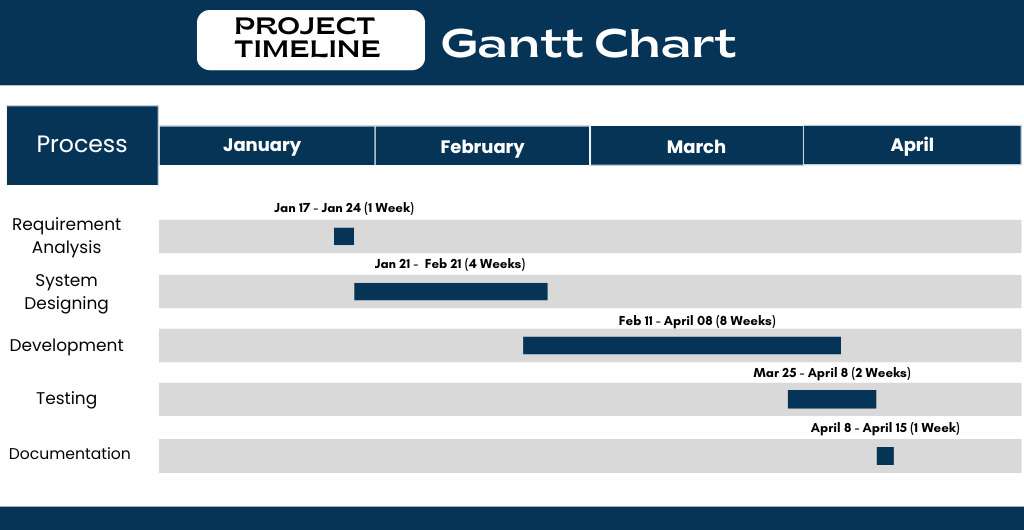
\includegraphics[width=0.90\textwidth]{Images/Project Timeline.jpg}
\caption{Project Timeline}
\end{figure}
\FloatBarrier



\begin{figure}[h]
\centering
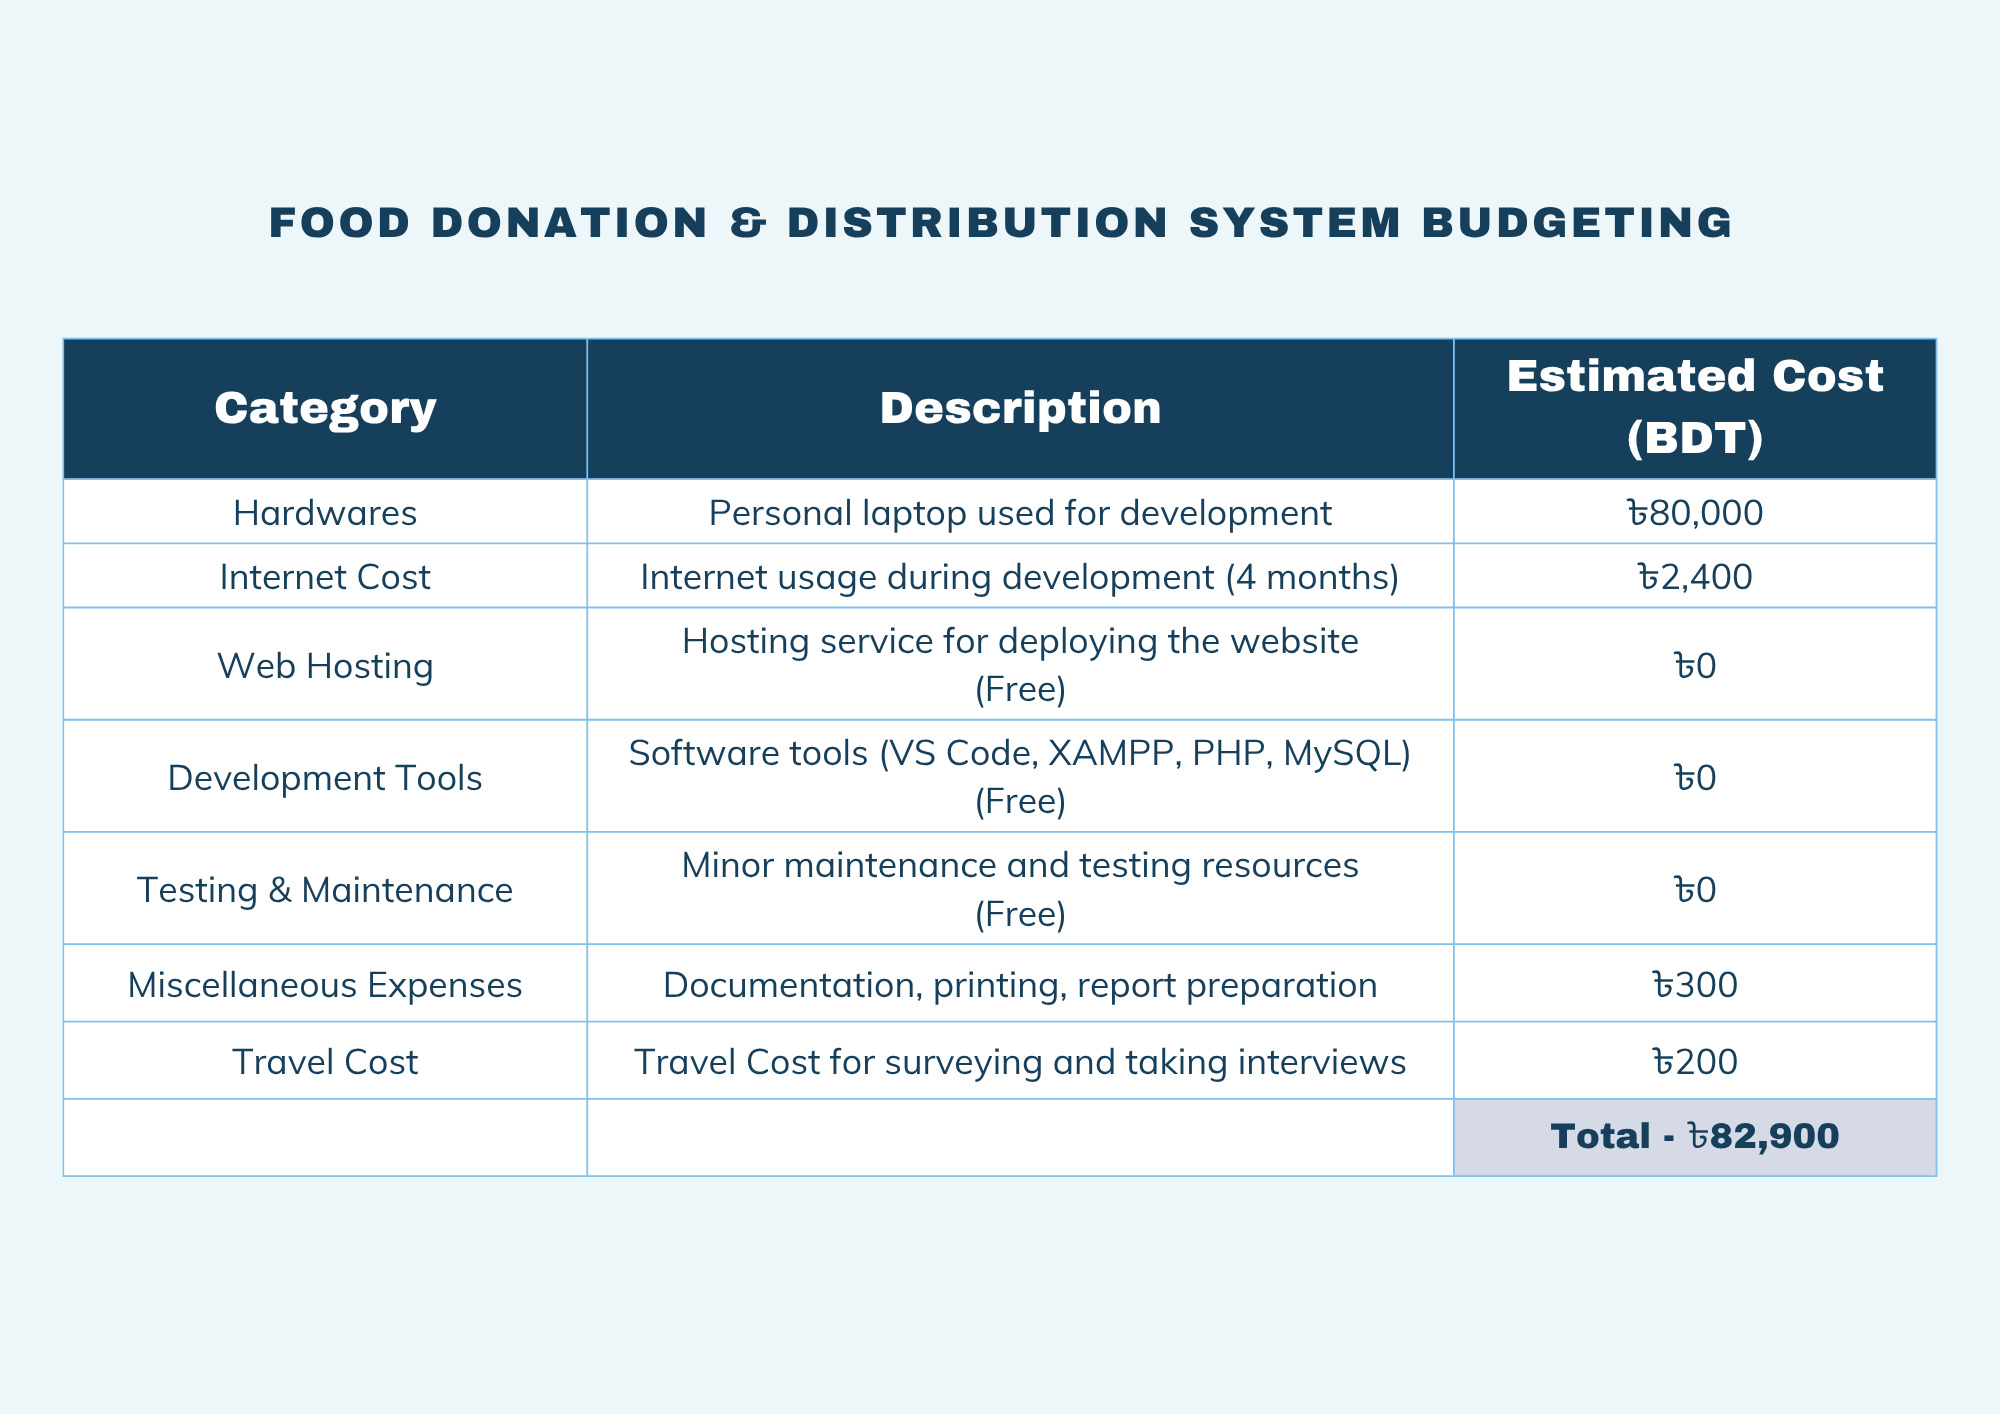
\includegraphics[width=0.90\textwidth]{Images/Budget.jpg}
\caption{Estimated Project Budget}
\end{figure}
\FloatBarrier









\section{Technical Requirements}
\textbf{Tools/Hardware Requirements:}
\begin{itemize}
    \item Computer/Laptop
    \item Internet connection
    \item Web browser
\end{itemize}

 \vspace{10pt}
\textbf{Technologies/Software Requirements:}
\begin{itemize}
    \item Backend: PHP
    \item Frontend: HTML, CSS
    \item Database: MySQL, phpMyAdmin
    \item Web Server: Apache / XAMPP
    \item Development Tools: Visual Studio Code
    \item Web Browser: Google Chrome, Firefox
\end{itemize}




 \vspace{30pt}
\section{Functional Requirements}

The system should provide the following functions:

\textbf{User:}
\begin{itemize}
    \item Register
    \item Log In
    \item Log Out
\end{itemize}

 \vspace{15pt}
\textbf{Donor:}
\begin{itemize}
    \item Add food donation
    \item View donations details
\end{itemize}

\textbf{NGO:}
\begin{itemize}
    \item View available donations
    \item Search/filter available donations
    \item Request donations
    \item View/track my requests
\end{itemize}

 \vspace{10pt}
\textbf{Admin:}
\begin{itemize}
    \item View all requests
    \item Sort/filter requests
    \item Approve requests
    \item Reject requests
\end{itemize}






 \vspace{50pt}
\section{Non-Functional Requirements}

\begin{itemize}
    \item \textbf{Usability:} Simple interface for easy interaction.
    \item \textbf{Security:} User authentication and protected database access.
    \item \textbf{Performance:} Fast loading pages and efficient queries.
    \item \textbf{Reliability:} The system should function consistently without errors.
    \item \textbf{Scalability:} The system should allow future expansion.
\end{itemize}





\vspace{80pt}
\section{System Design}
\subsection{Activity Diagram}
\begin{figure}[h]
\centering
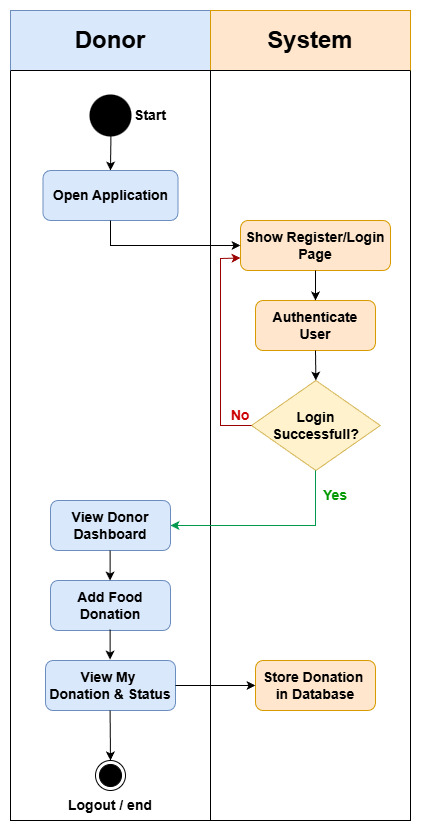
\includegraphics[width=0.50\textwidth]{Images/Donor Activity DIagram.jpg}

Donor Activity Diagram
\end{figure}
\FloatBarrier


\begin{figure}[h]
\centering
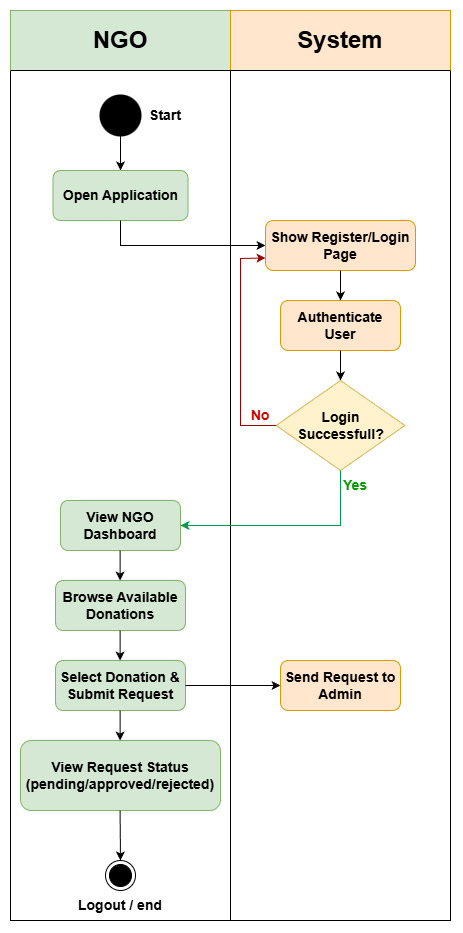
\includegraphics[width=0.60\textwidth]{Images/NGO Activity DIagram.jpg}

NGO Activity Diagram
\end{figure}
\FloatBarrier


\begin{figure}[h]
\centering
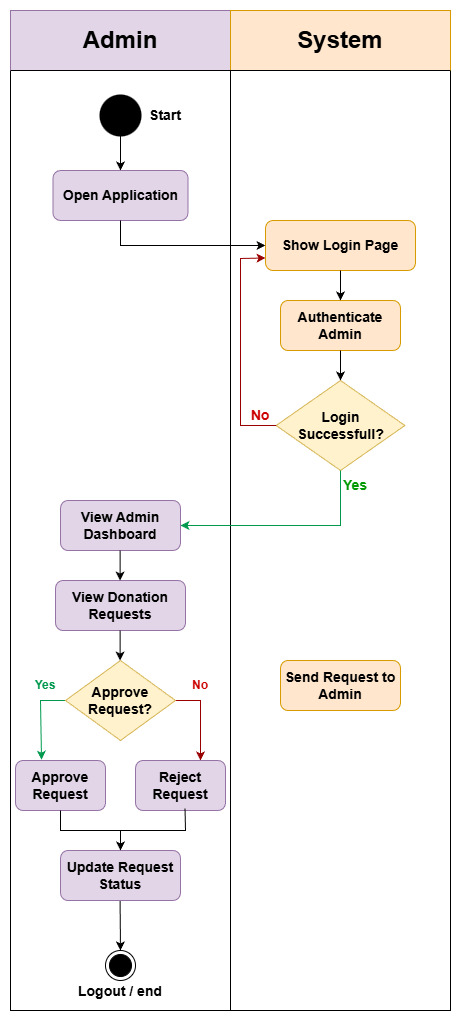
\includegraphics[width=0.60\textwidth]{Images/Admin Activity DIagram.jpg}

Admin Activity Diagram
\end{figure}
\FloatBarrier









\subsection{Use Case Diagram}
\begin{figure}[H]
\centering
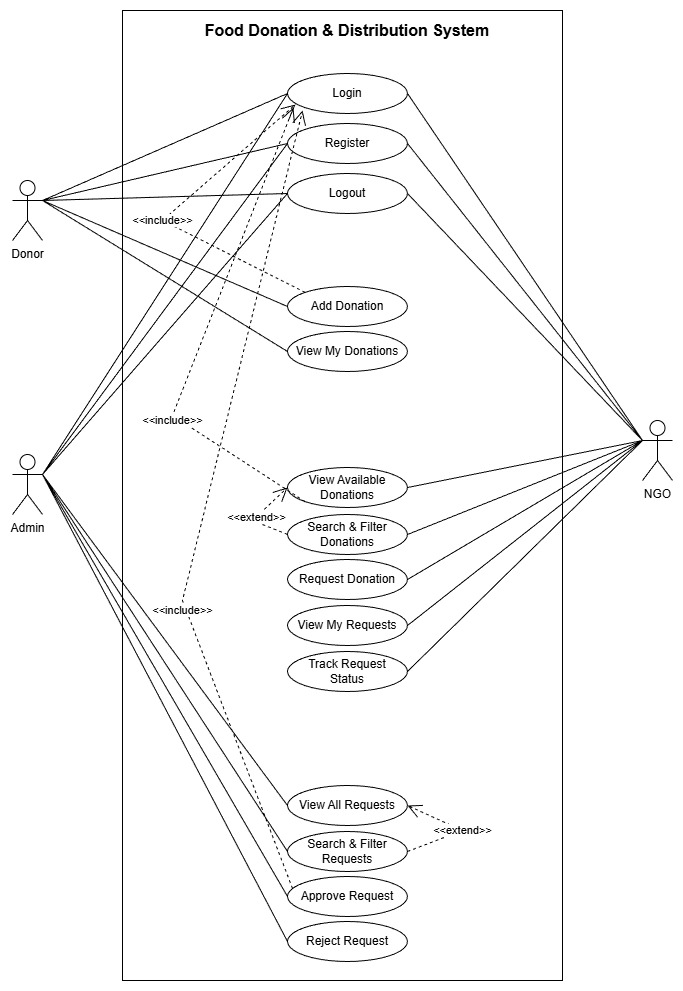
\includegraphics[width=0.8\textwidth]{Images/Dp Use Case.jpg}

Use Case Diagram
\end{figure}




 \vspace{20pt}
\subsection{UML Class Diagram}
\begin{figure}[h]
\centering
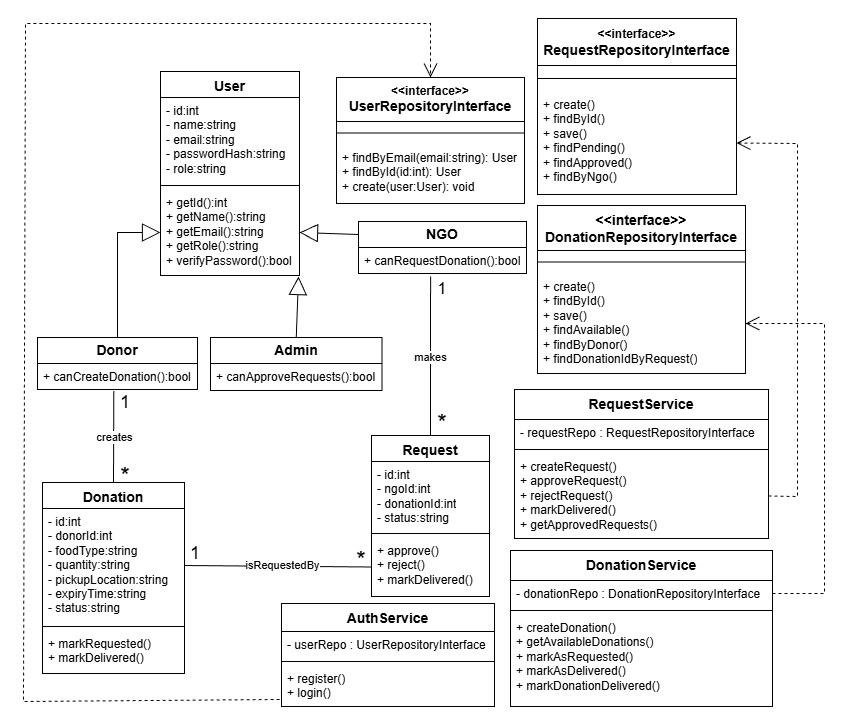
\includegraphics[width=1.0\textwidth]{Images/Dp Class Diagram.jpg}

UML Class Diagram of the System
\end{figure}
\FloatBarrier

 \vspace{140pt}
\subsection{System Sequence Diagram}
\begin{figure}[h]
\centering
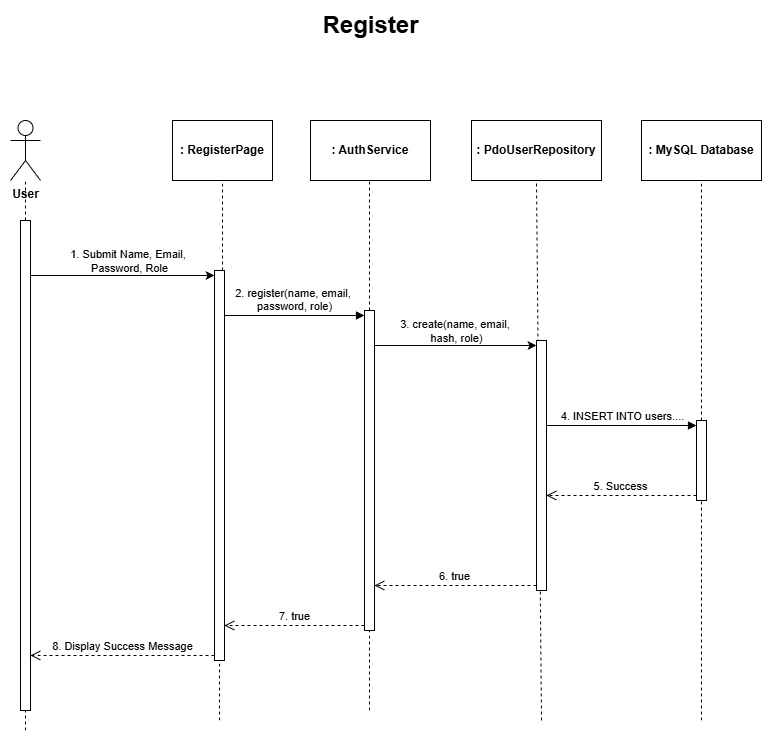
\includegraphics[width=\textwidth]{Images/Register.jpg}
\end{figure}
\FloatBarrier

\begin{figure}[h]
\centering
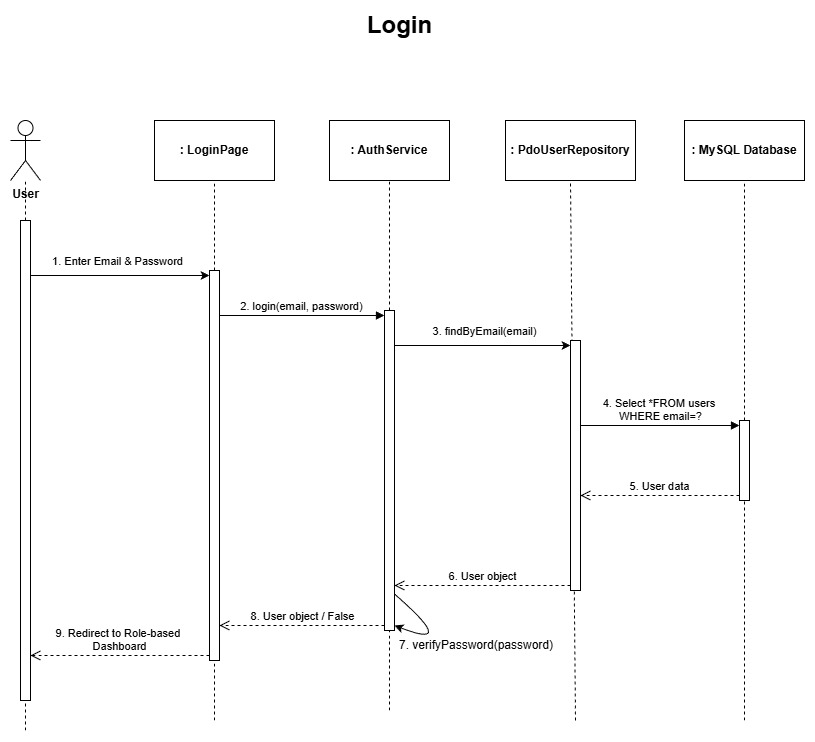
\includegraphics[width=\textwidth]{Images/Login.jpg}
\end{figure}
\FloatBarrier

\begin{figure}[h]
\centering
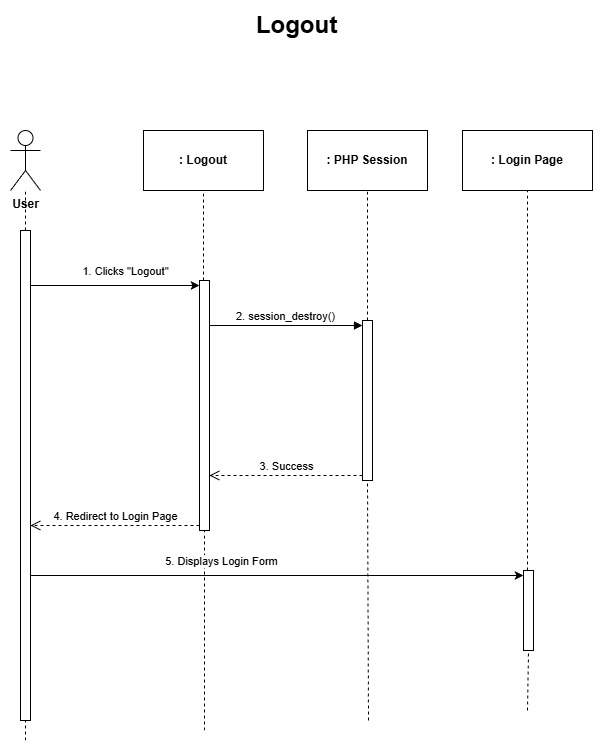
\includegraphics[width=\textwidth]{Images/Logout.jpg}
\end{figure}
\FloatBarrier

\begin{figure}[h]
\centering
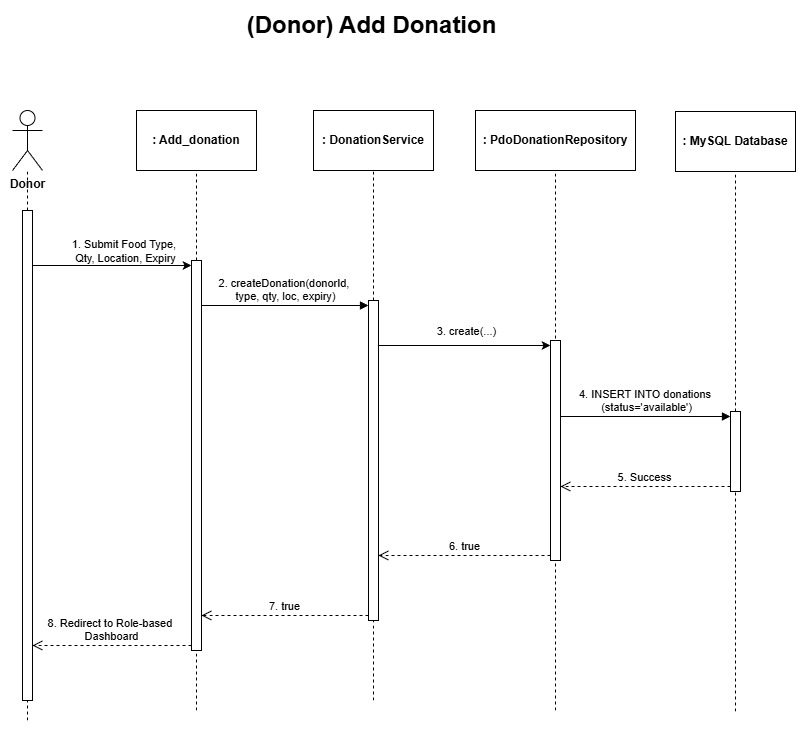
\includegraphics[width=\textwidth]{Images/(Donor) Add Donation.jpg}
\end{figure}
\FloatBarrier

\begin{figure}[h]
\centering
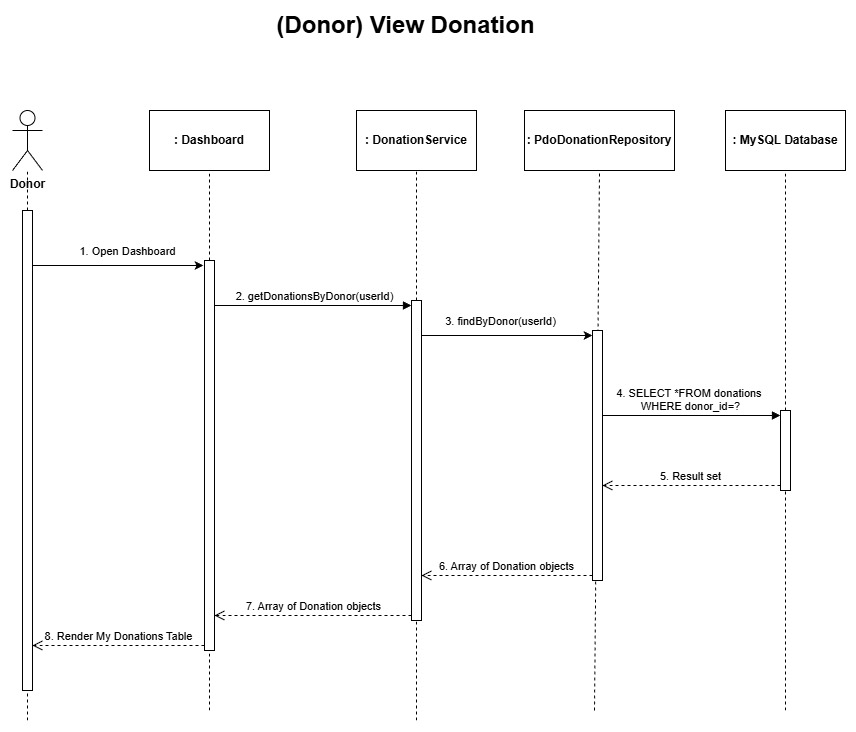
\includegraphics[width=\textwidth]{Images/(Donor) View Donation.jpg}
\end{figure}
\FloatBarrier

\begin{figure}[h]
\centering
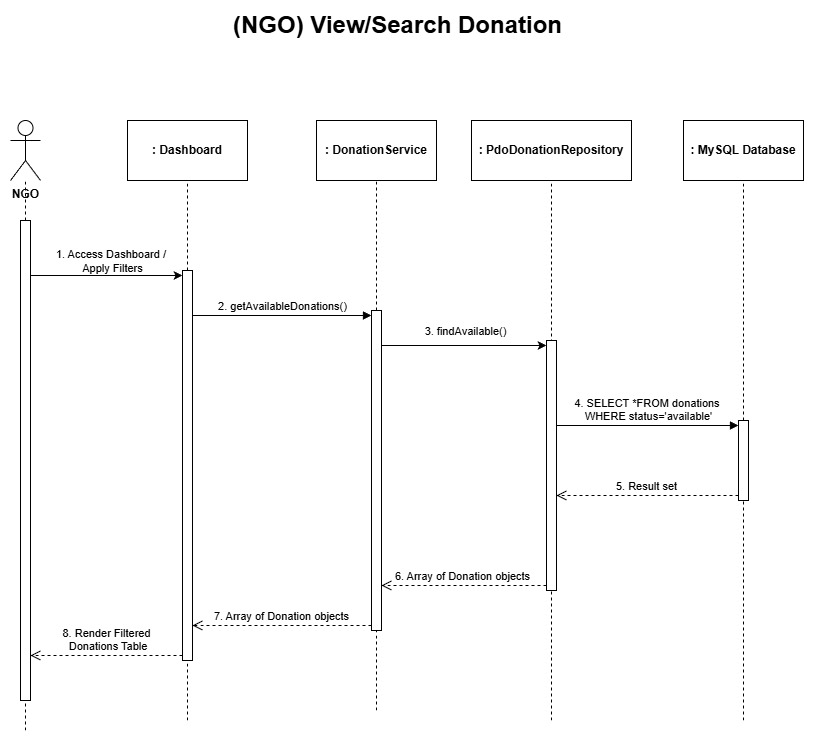
\includegraphics[width=\textwidth]{Images/(NGO) View or search Donation.jpg}
\end{figure}
\FloatBarrier

\begin{figure}[h]
\centering
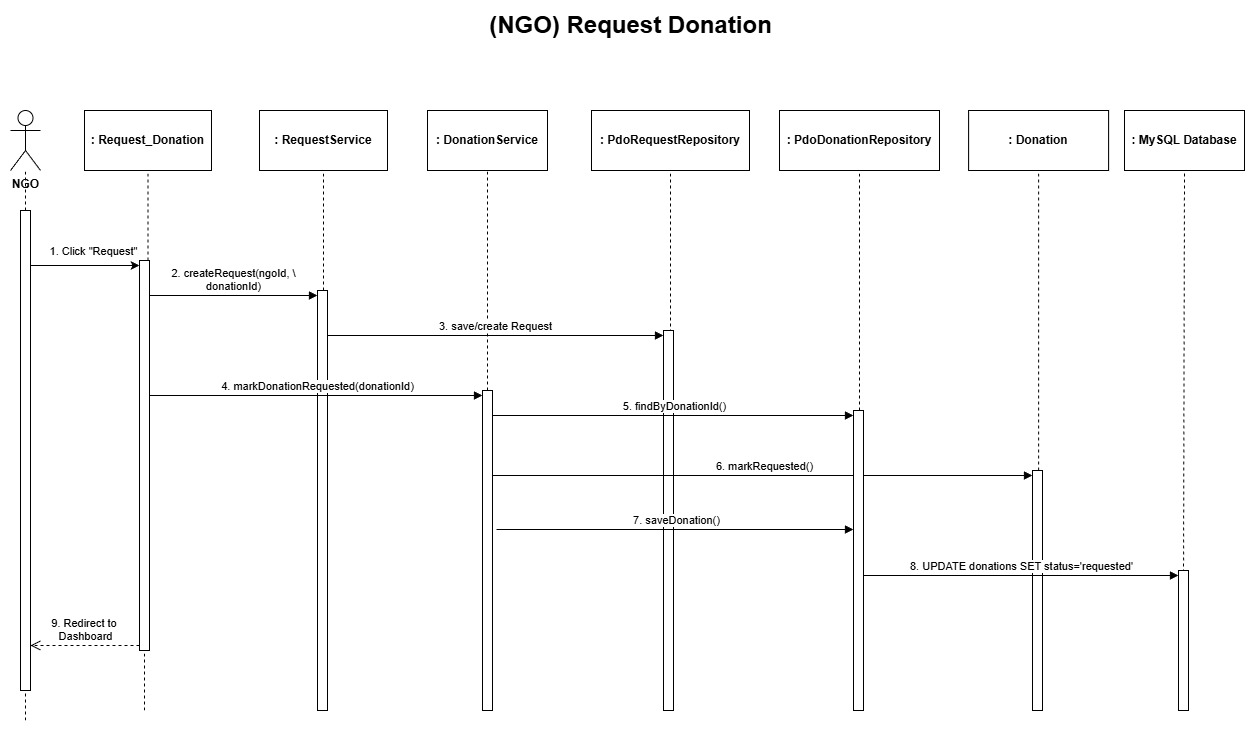
\includegraphics[width=\textwidth]{Images/(NGO) Req Donation.jpg}
\end{figure}
\FloatBarrier

\begin{figure}[h]
\centering
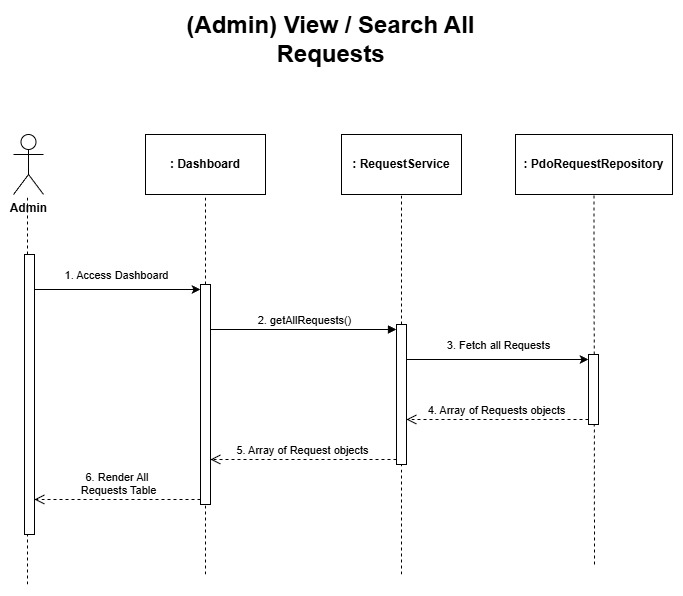
\includegraphics[width=\textwidth]{Images/(Admin) View or Search Req.jpg}
\end{figure}
\FloatBarrier

\begin{figure}[h]
\centering
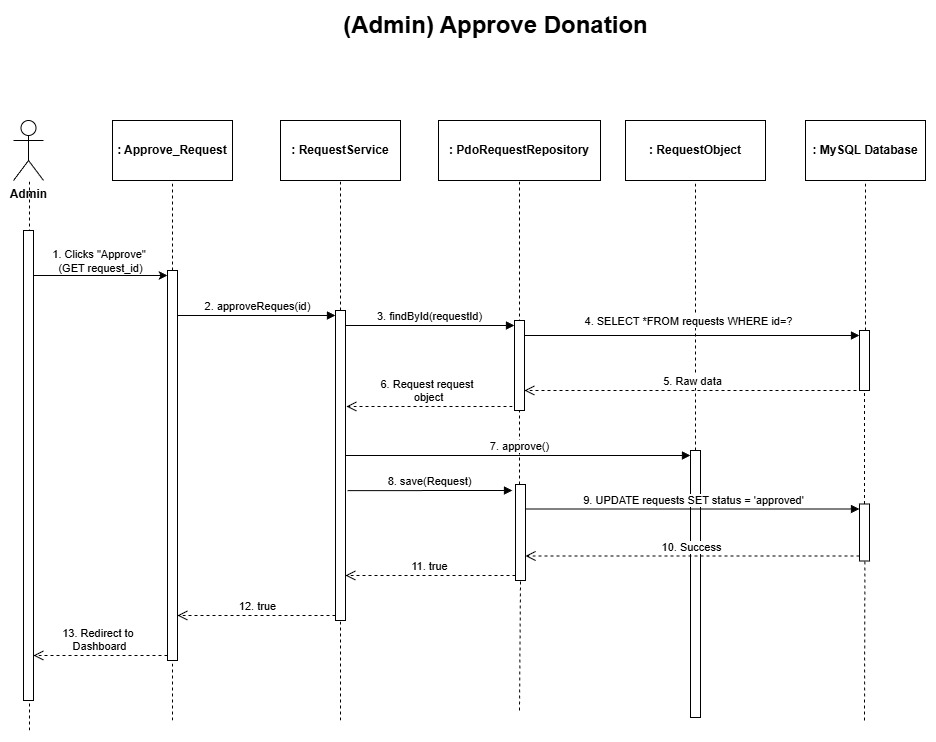
\includegraphics[width=\textwidth]{Images/(Admin) Approve Req.jpg}
\end{figure}
\FloatBarrier

\begin{figure}[h]
\centering
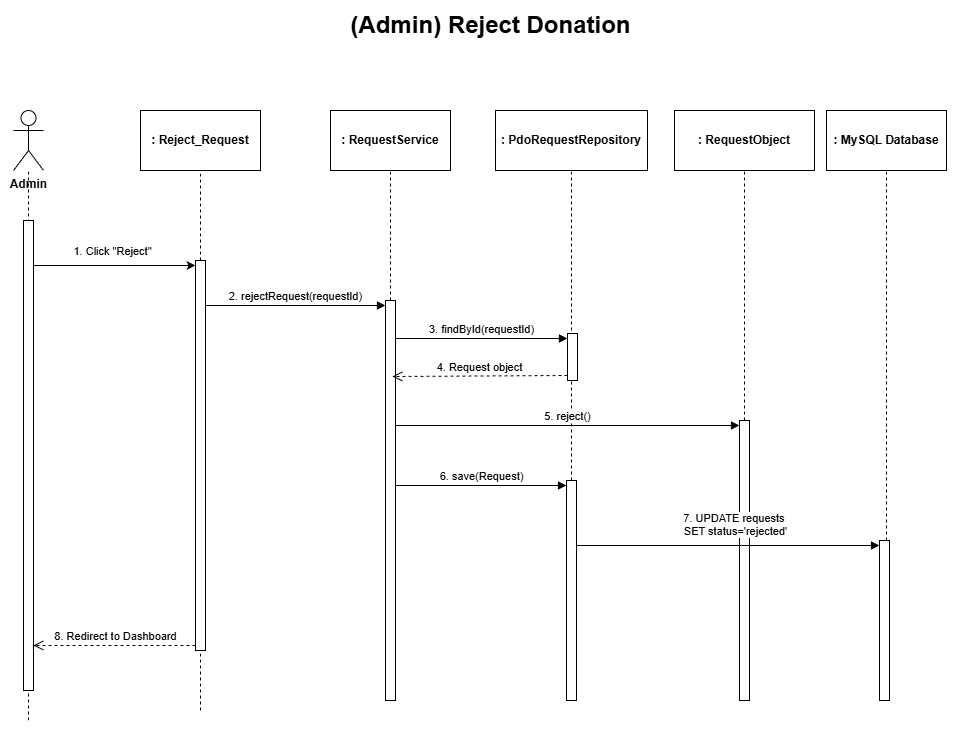
\includegraphics[width=\textwidth]{Images/(Admin) Reject Req.jpg}
\end{figure}
\FloatBarrier




\section{Development Methodology}

The Food Donation Management System was developed using the Waterfall Software Development Model. The Waterfall model is a sequential development approach where each phase of the project is completed before moving to the next phase. This model provides a structured process for planning, designing, developing, and testing the system.

The following stages were followed during the development of this project:

 \vspace{20pt}
\textbf{1. Requirement Analysis - }In this phase, the requirements of the system were identified and analyzed. Information about the problems related to food waste and food donation was collected through research and surveys. The system requirements for different users such as donors, NGOs, and administrators were defined, including features like user registration, food donation submission, and request management.

 \vspace{20pt}
\textbf{2. System Design-} During this phase, the overall structure of the system was planned. System diagrams such as Activity Diagram, Use Case Diagram, UML Class Diagram, and System Sequence Diagram were designed to represent the workflow and interactions within the system. The database structure was also designed to store user, donation, and request information.

 \vspace{20pt}
\textbf{3. Implementation -} In the implementation phase, the actual development of the system was carried out. The application was developed using PHP for backend development, MySQL for database management, and HTML and CSS for the user interface. Different modules such as the donor dashboard, NGO request system, and admin panel were developed.

 \vspace{20pt}
\textbf{4. Testing -} After development, the system was tested to ensure that all features worked correctly. Testing included checking the login system, donation submission process, and request management to ensure the system met the required functionality.

 \vspace{20pt}
\textbf{5. Deployment and Maintenance -} Finally, the system was deployed in a local server environment using XAMPP. Future maintenance may include fixing errors, improving the user interface, and adding new features to enhance the system.


The Waterfall model helped ensure that the project followed a clear and organized development process from requirement analysis to final deployment.

 \vspace{10pt}
\begin{figure}[h]
\centering
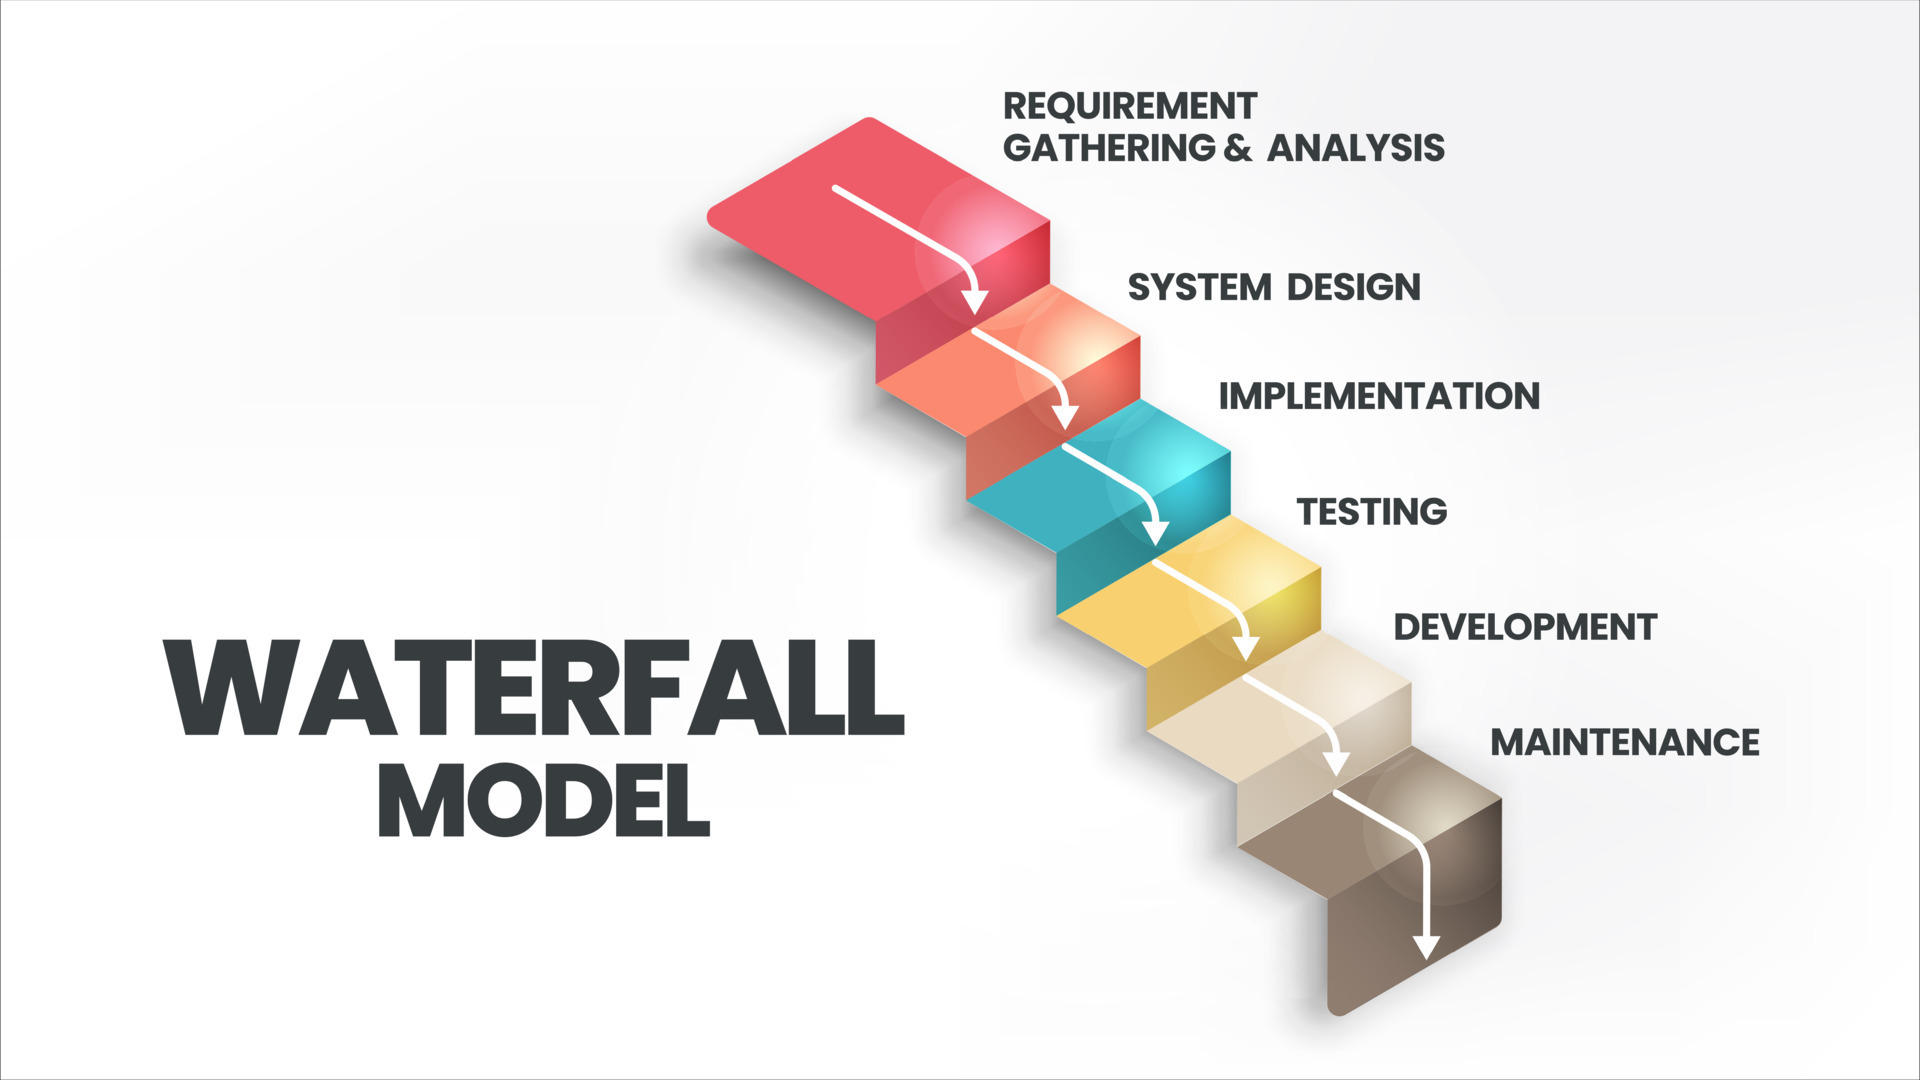
\includegraphics[width=0.90\textwidth]{Images/waterfall1.jpg}
\end{figure}
\FloatBarrier






\section{Implementation (Screenshots of the Software)}


\begin{figure}[h]
\centering
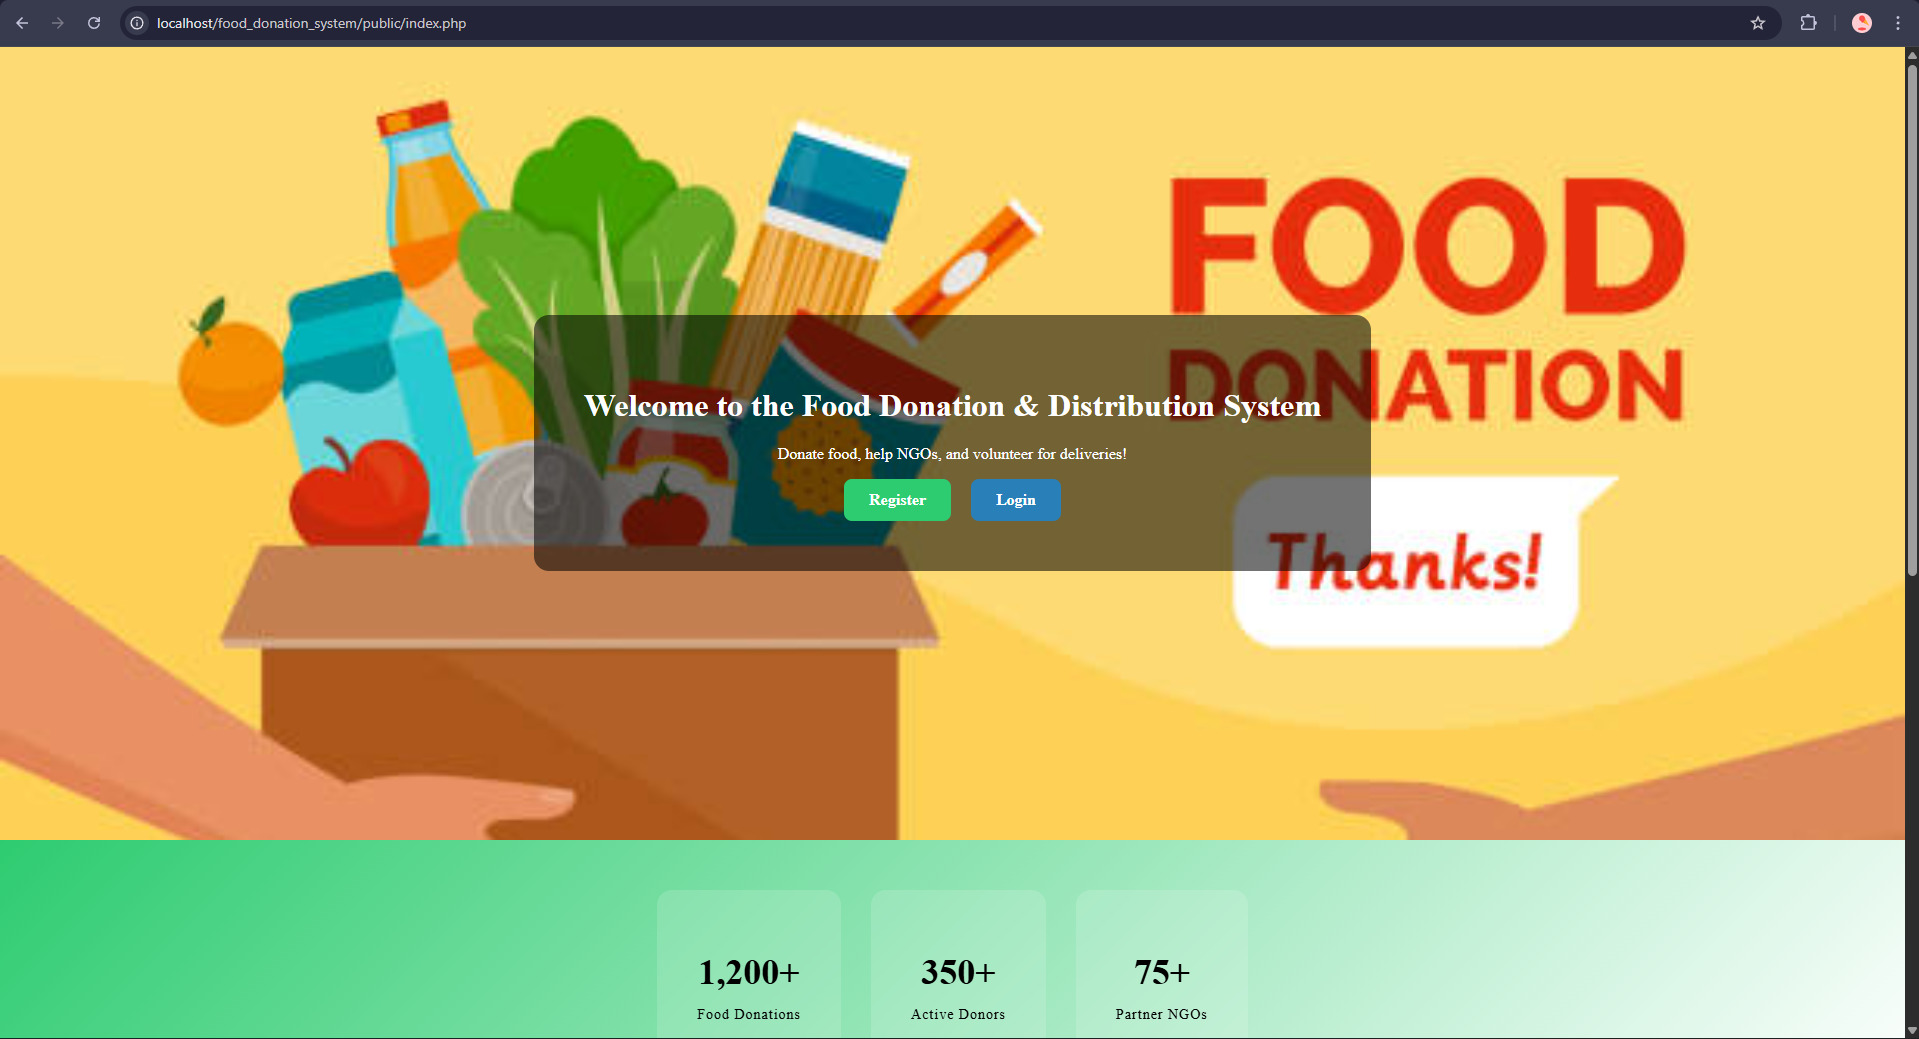
\includegraphics[width=0.90\textwidth]{Images/1. Public Dashboard.jpg}

Public Dashboard
\end{figure}
\FloatBarrier

\begin{figure}[h]
\centering
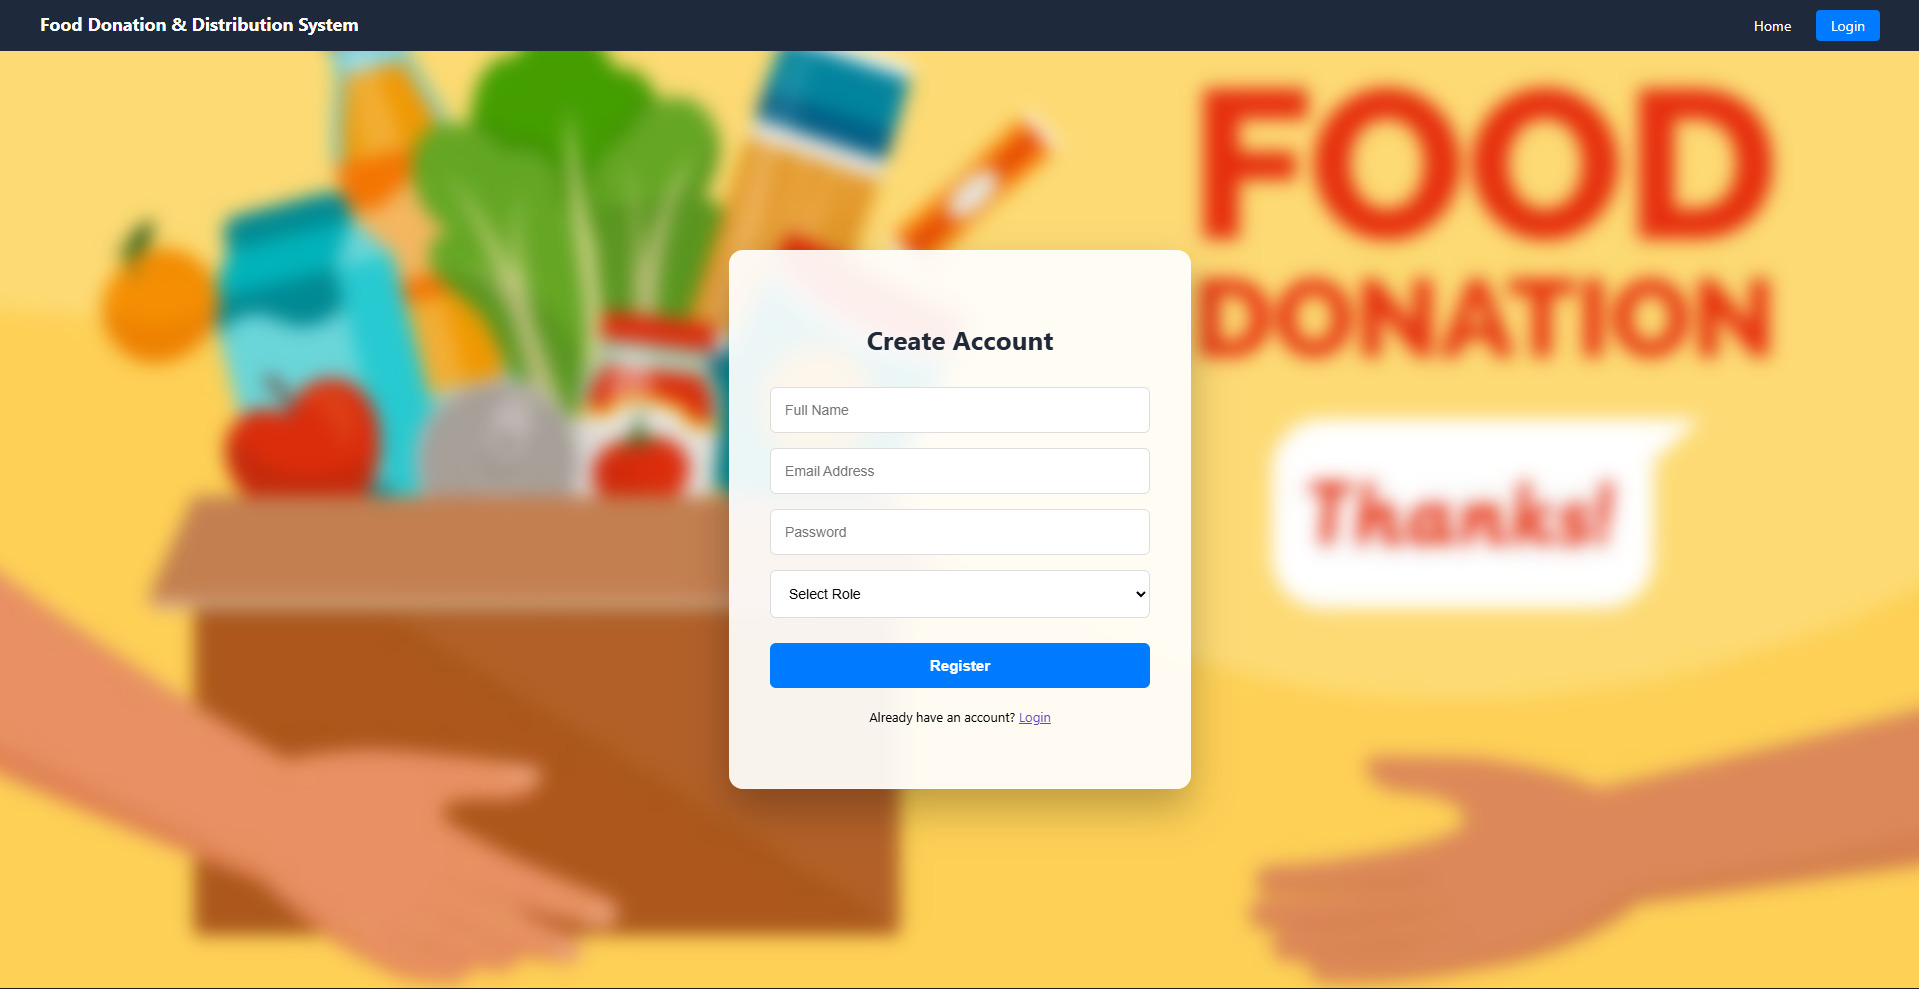
\includegraphics[width=0.90\textwidth]{Images/2. Registration Page.jpg}

Registration Page
\end{figure}
\FloatBarrier

\begin{figure}[h]
\centering
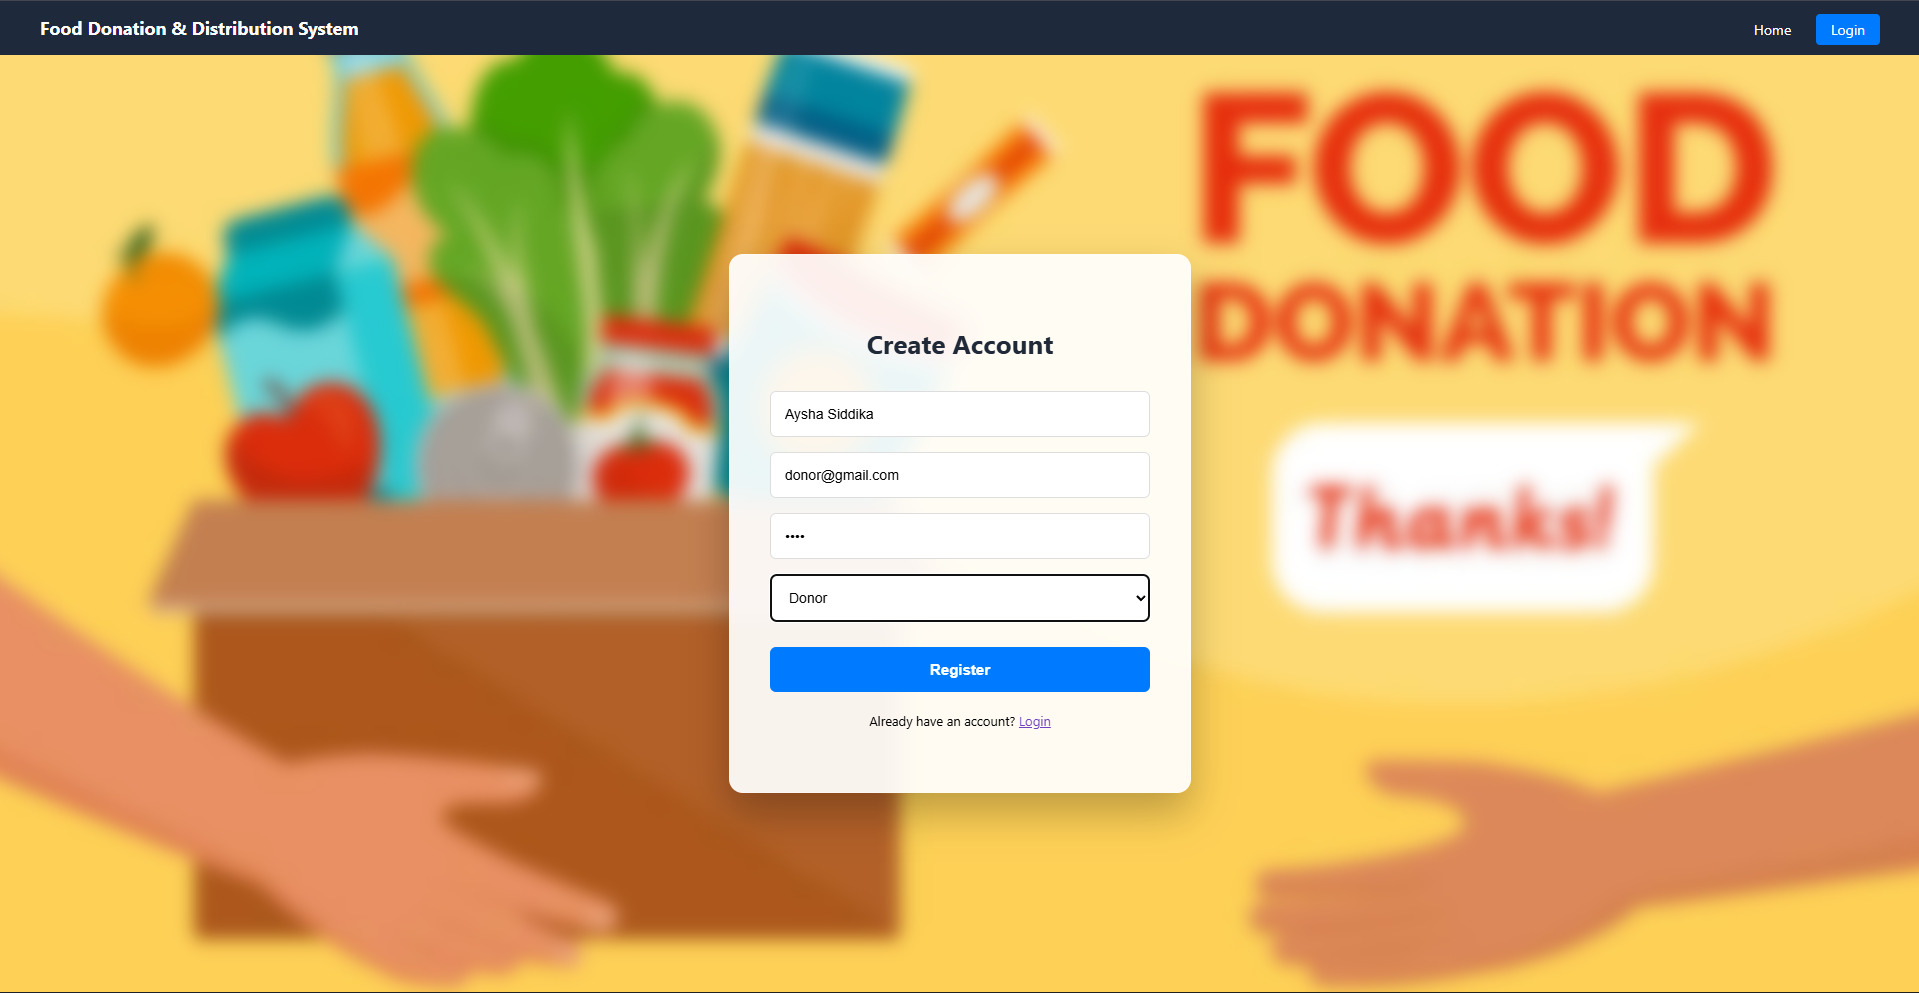
\includegraphics[width=0.90\textwidth]{Images/3. Registration as Donor.jpg}

Registration as Donor
\end{figure}
\FloatBarrier

\begin{figure}[h]
\centering
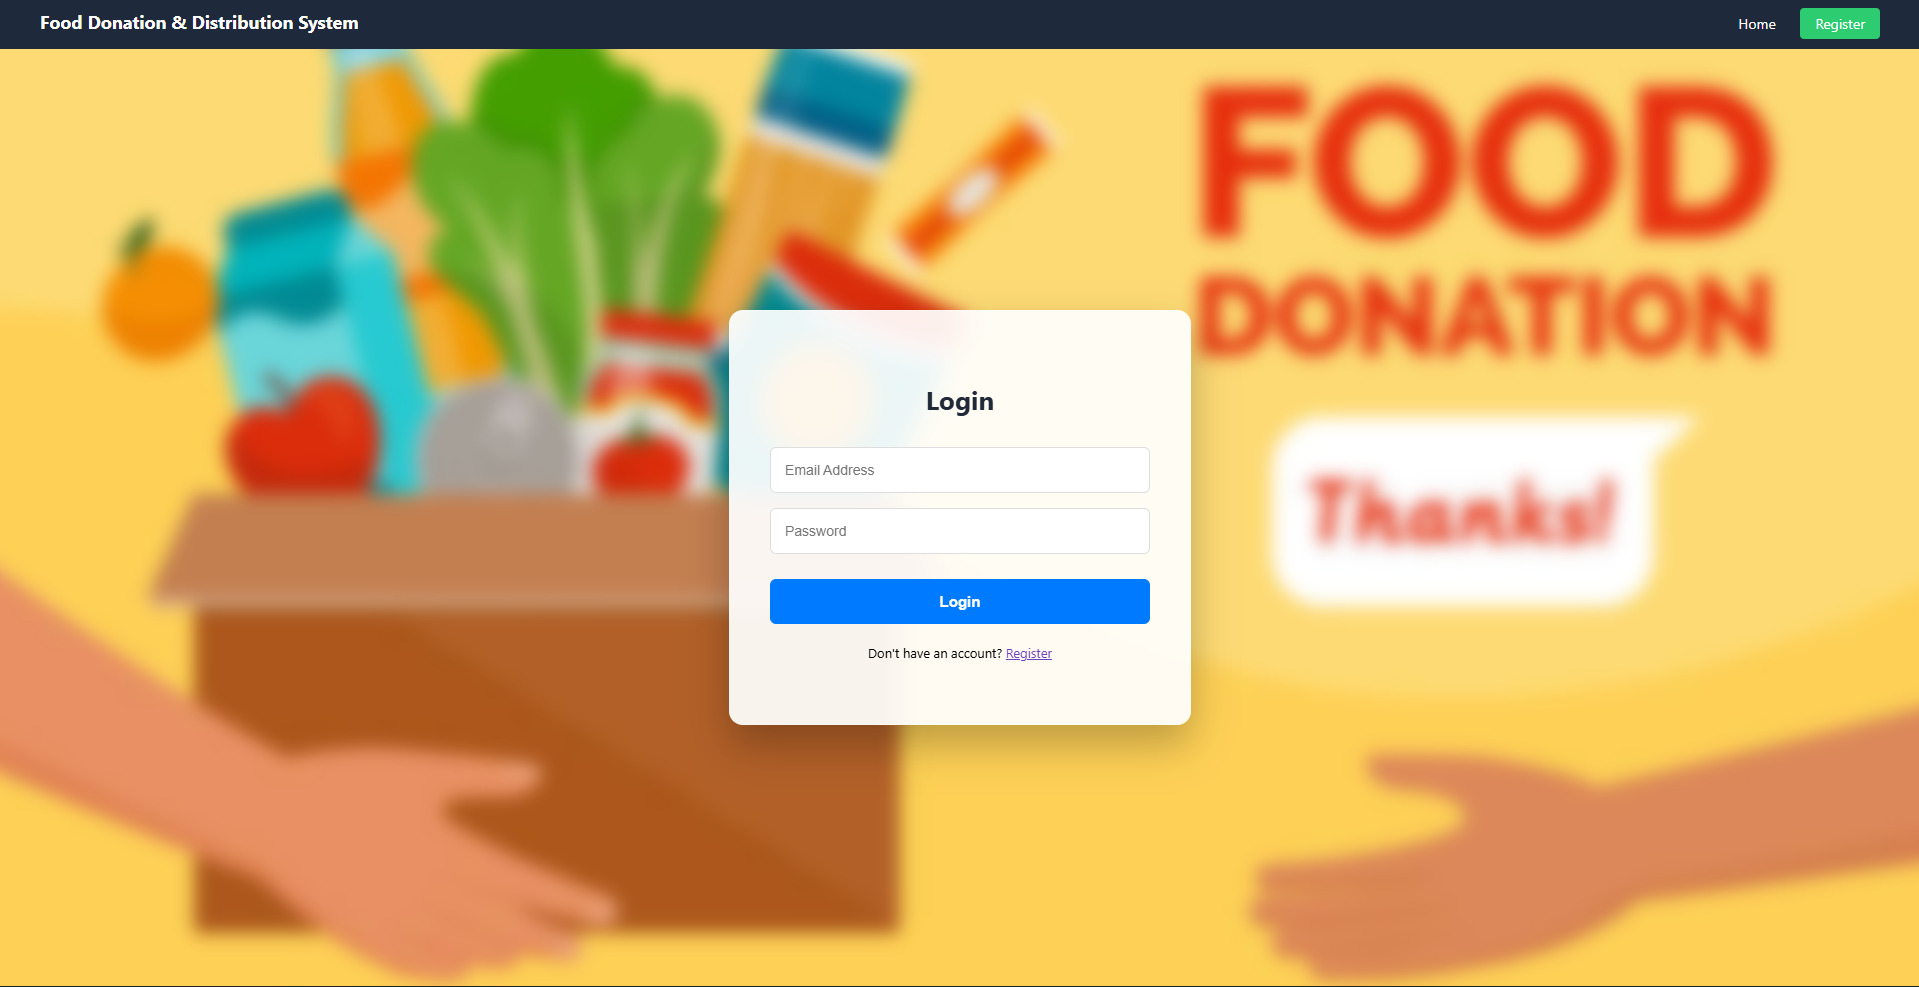
\includegraphics[width=0.90\textwidth]{Images/4. Login Page.jpg}

Login Page
\end{figure}
\FloatBarrier

\begin{figure}[h]
\centering
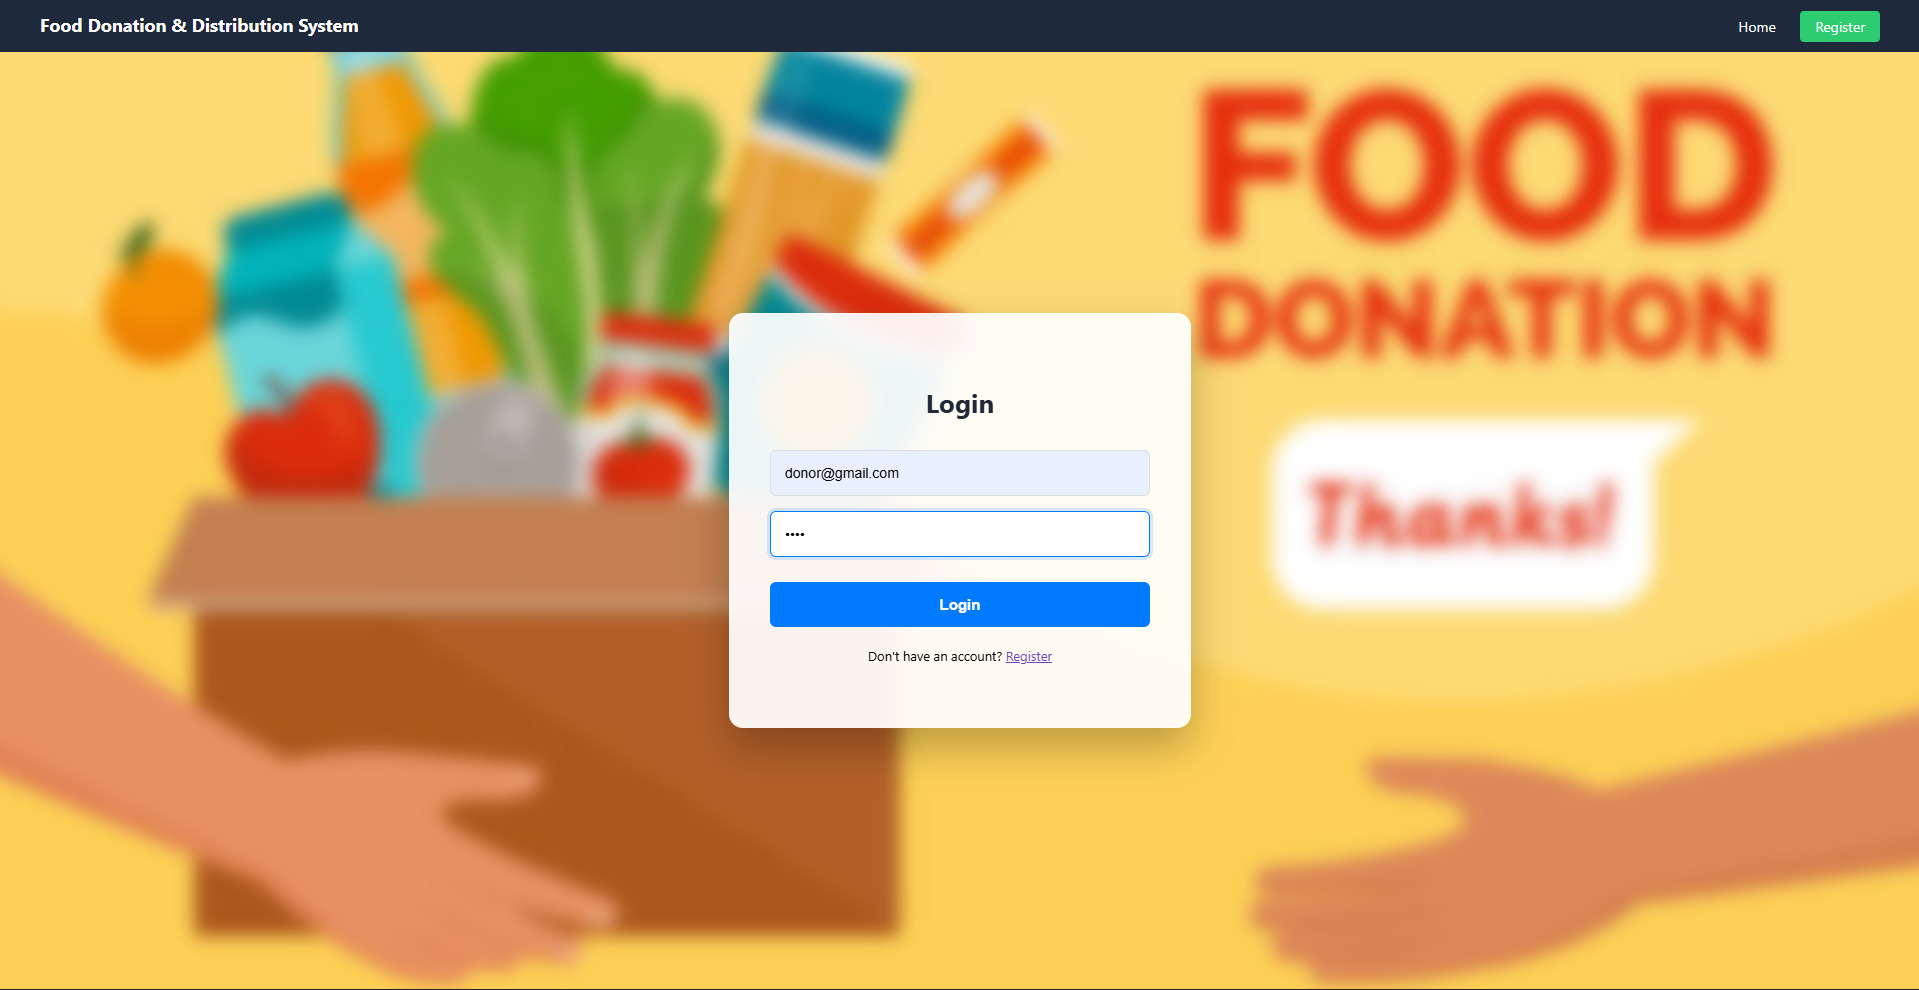
\includegraphics[width=0.90\textwidth]{Images/5. Login as Donor.jpg}

Login as Donor
\end{figure}
\FloatBarrier

\begin{figure}[h]
\centering
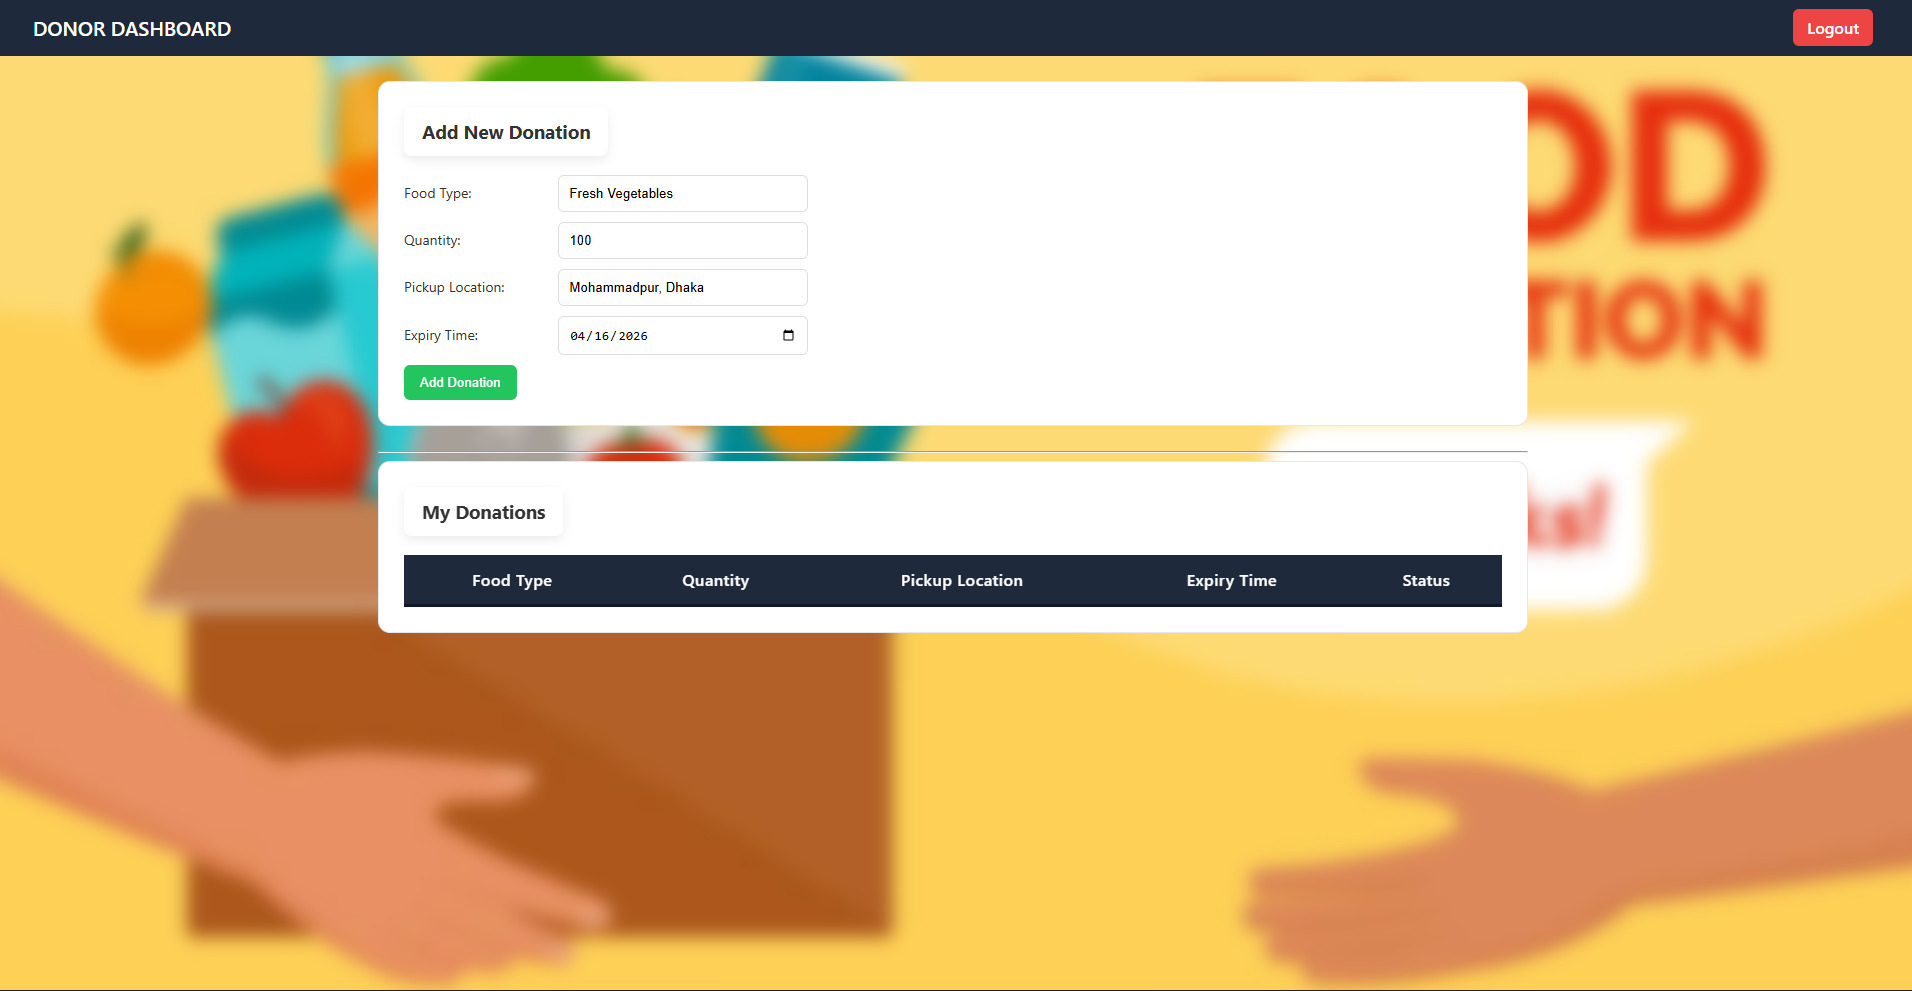
\includegraphics[width=0.90\textwidth]{Images/6. Donor Dashboard.jpg}

Donor Dashboard
\end{figure}
\FloatBarrier

\begin{figure}[h]
\centering
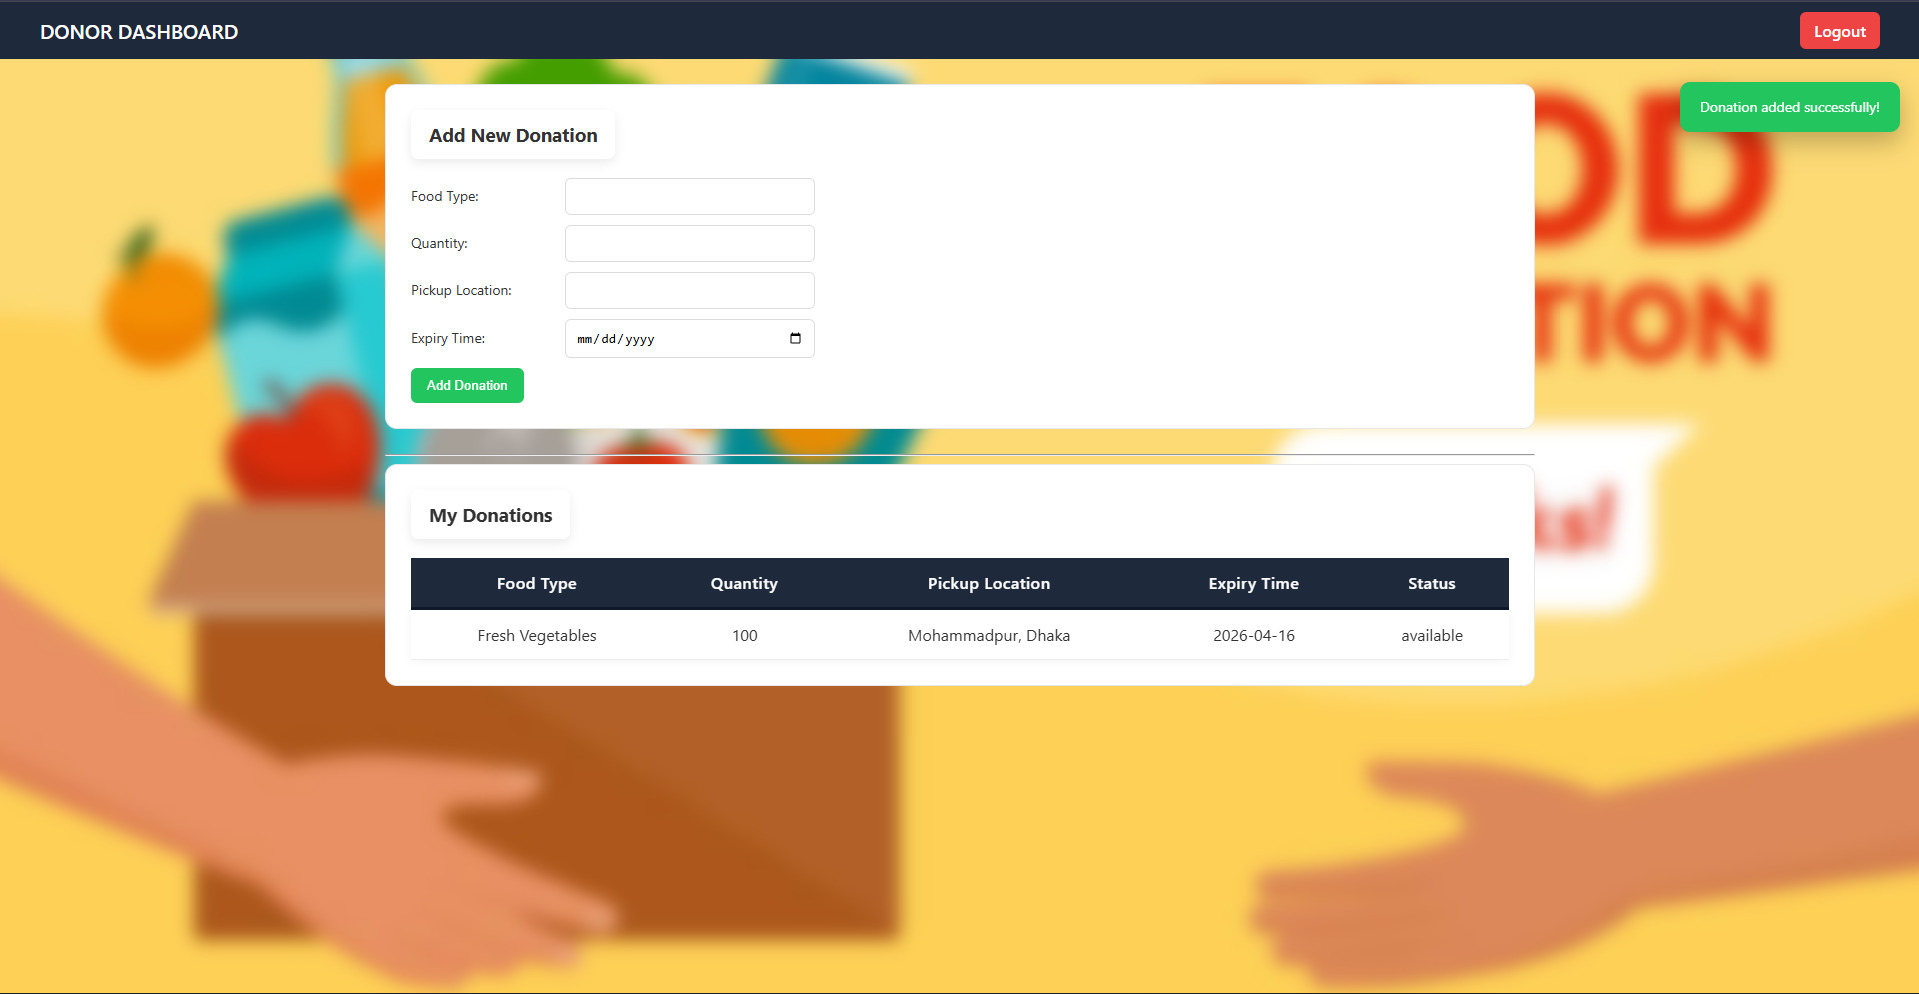
\includegraphics[width=0.90\textwidth]{Images/7. Donation Added.jpg}

Donation Added
\end{figure}
\FloatBarrier

\begin{figure}[h]
\centering
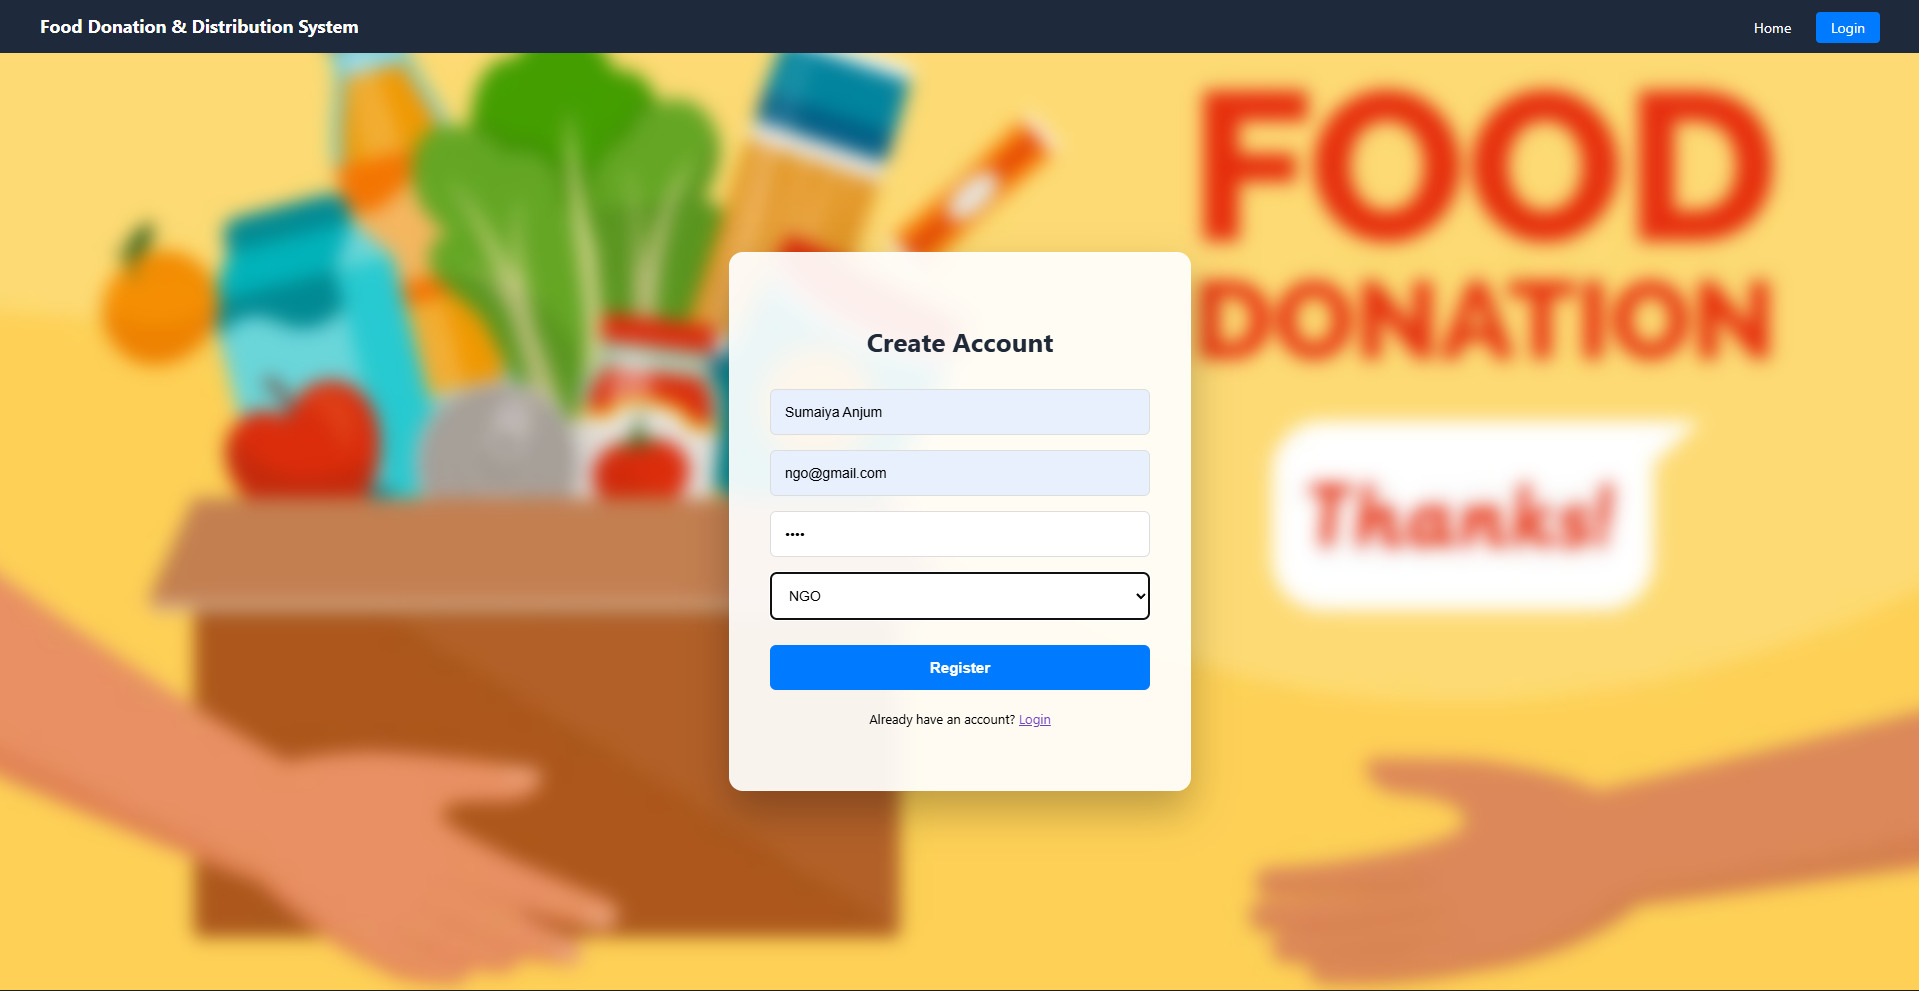
\includegraphics[width=0.90\textwidth]{Images/8. NGO Registration.jpg}

NGO Registration
\end{figure}
\FloatBarrier

\begin{figure}[h]
\centering
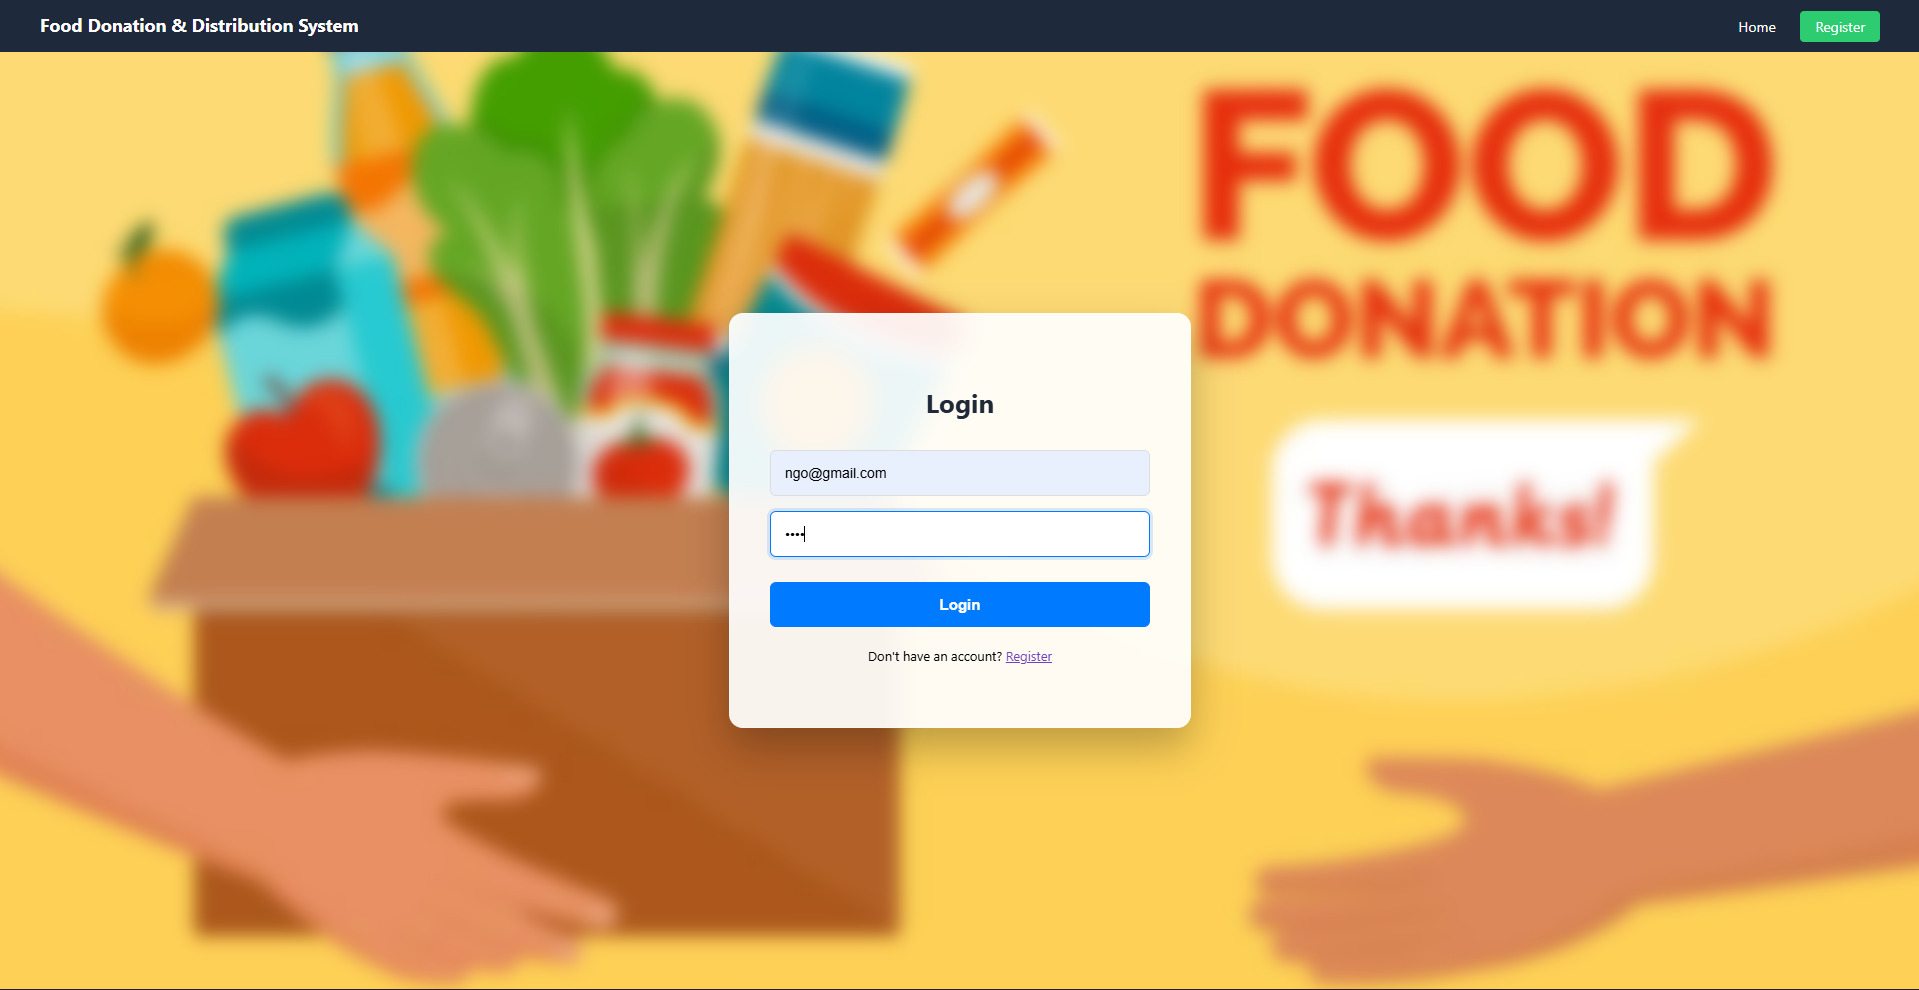
\includegraphics[width=0.90\textwidth]{Images/9. Login as NGO.jpg}

Login as NGO
\end{figure}
\FloatBarrier

\begin{figure}[h]
\centering
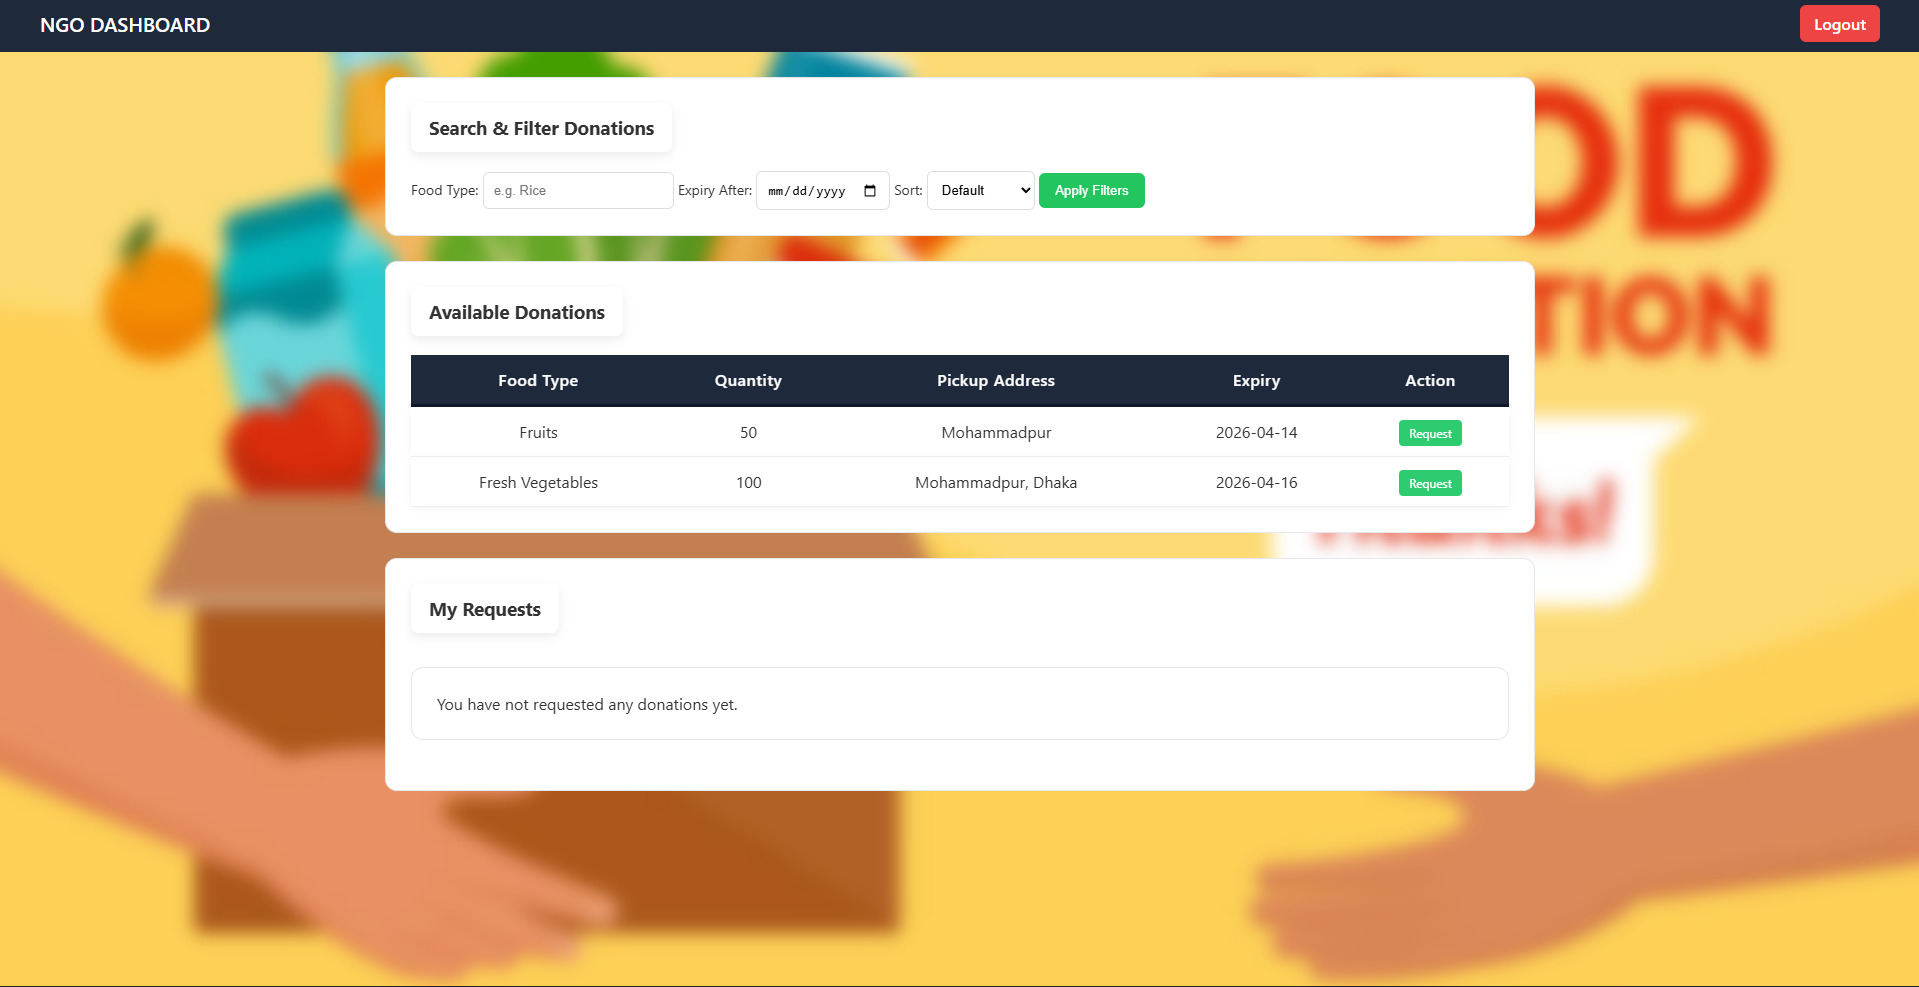
\includegraphics[width=0.90\textwidth]{Images/10. NGO Dashboard.jpg}

NGO Dashboard
\end{figure}
\FloatBarrier

\begin{figure}[h]
\centering
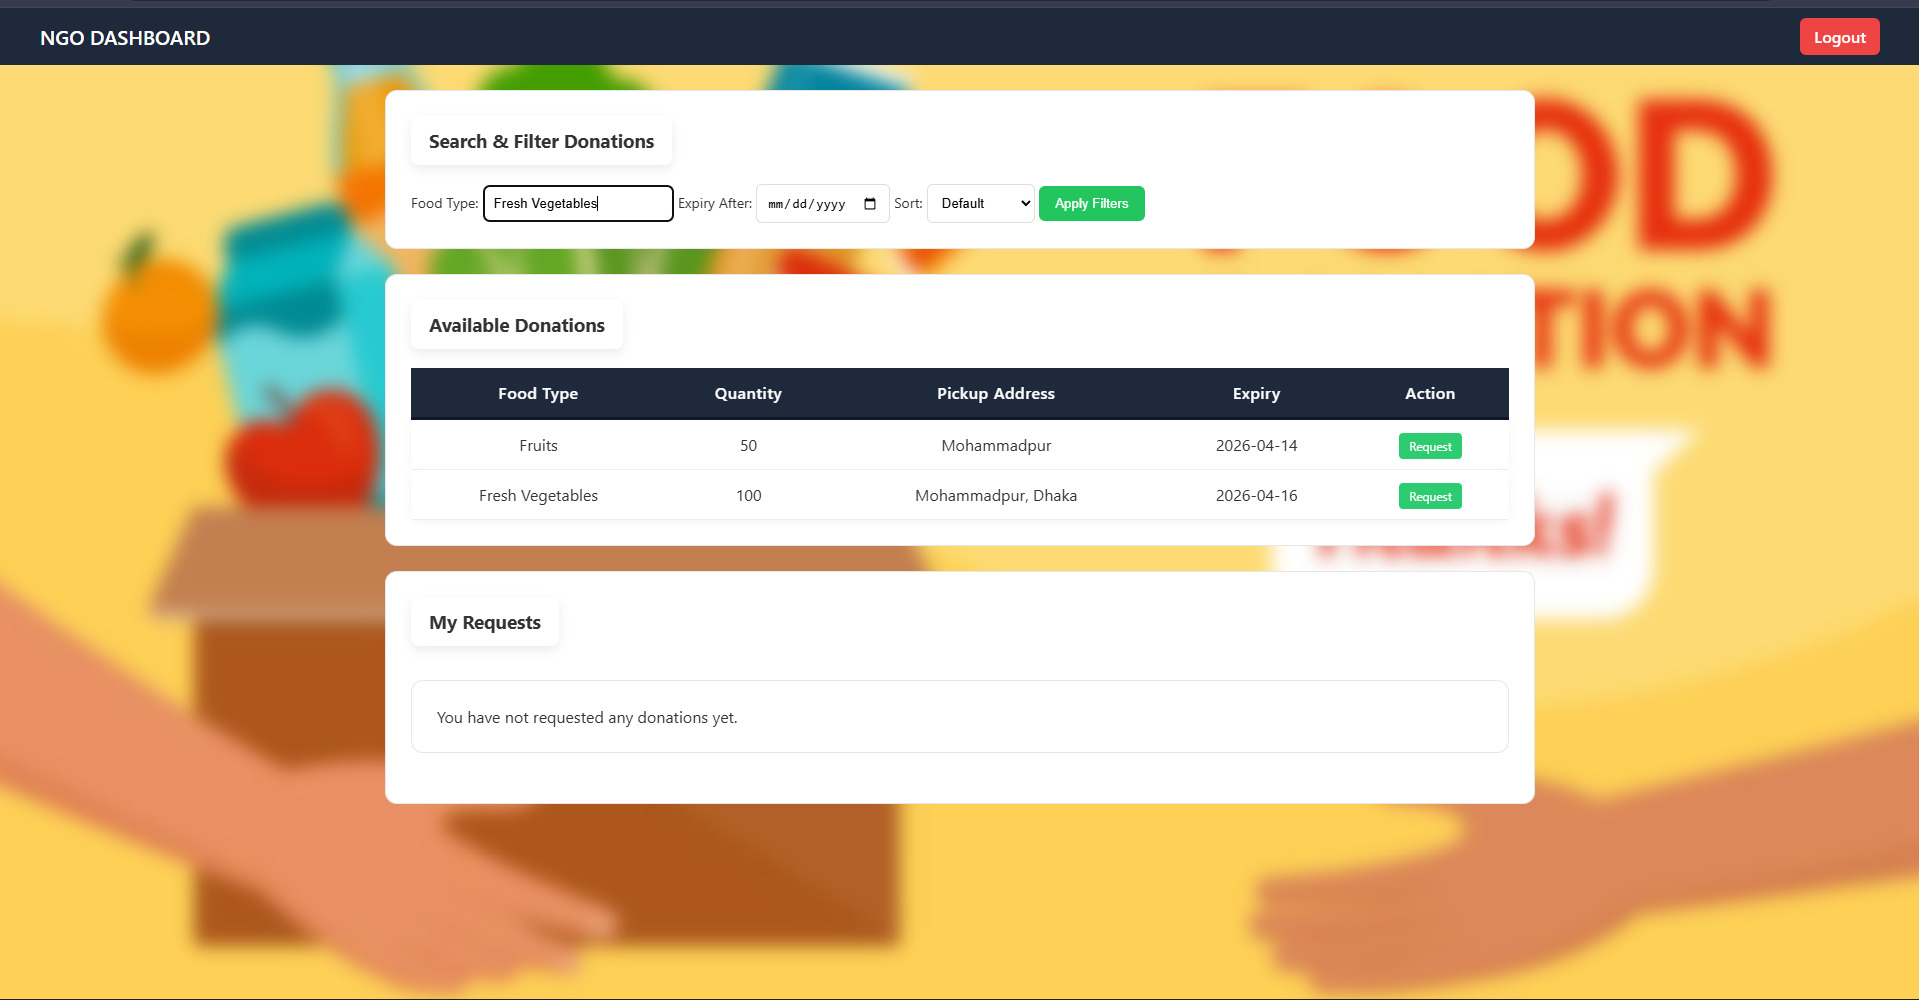
\includegraphics[width=0.90\textwidth]{Images/11. Search Available Donation by Food Type.jpg}

Search Available Donation by Food Type
\end{figure}
\FloatBarrier

\begin{figure}[h]
\centering
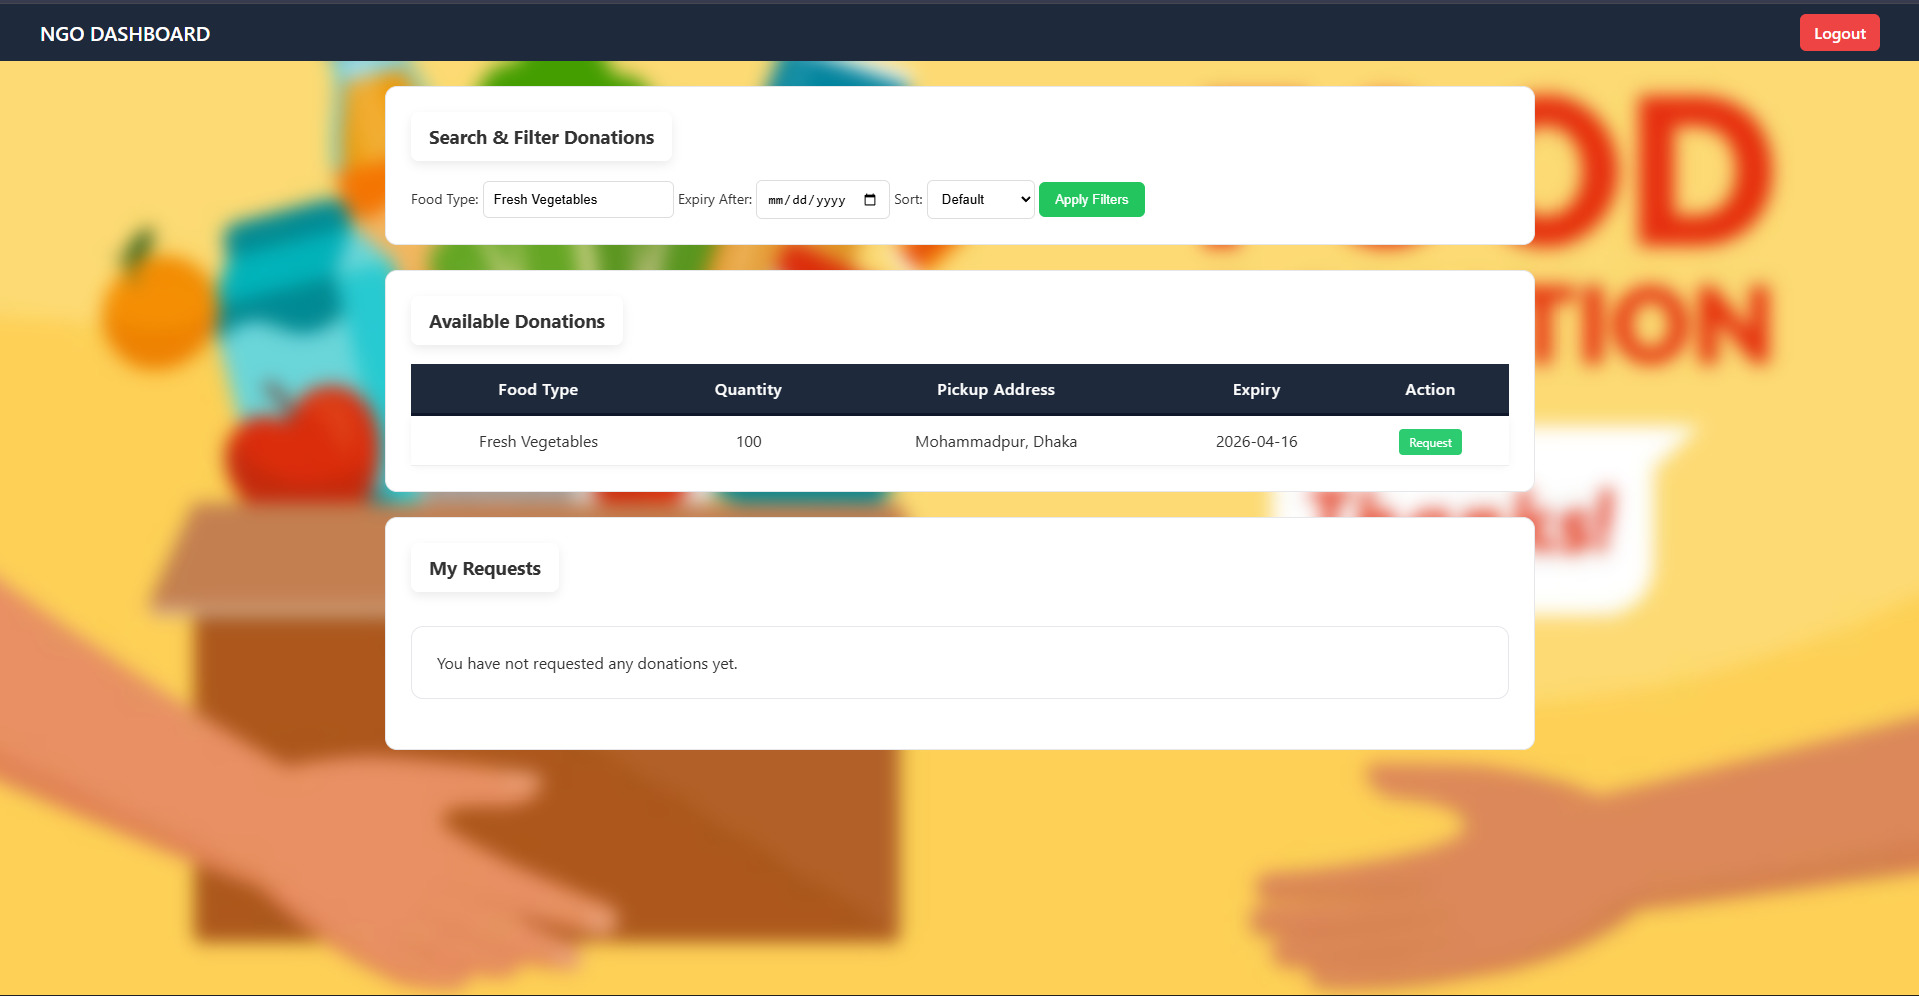
\includegraphics[width=0.90\textwidth]{Images/12. Search Result.jpg}

Search Result
\end{figure}
\FloatBarrier

\begin{figure}[h]
\centering
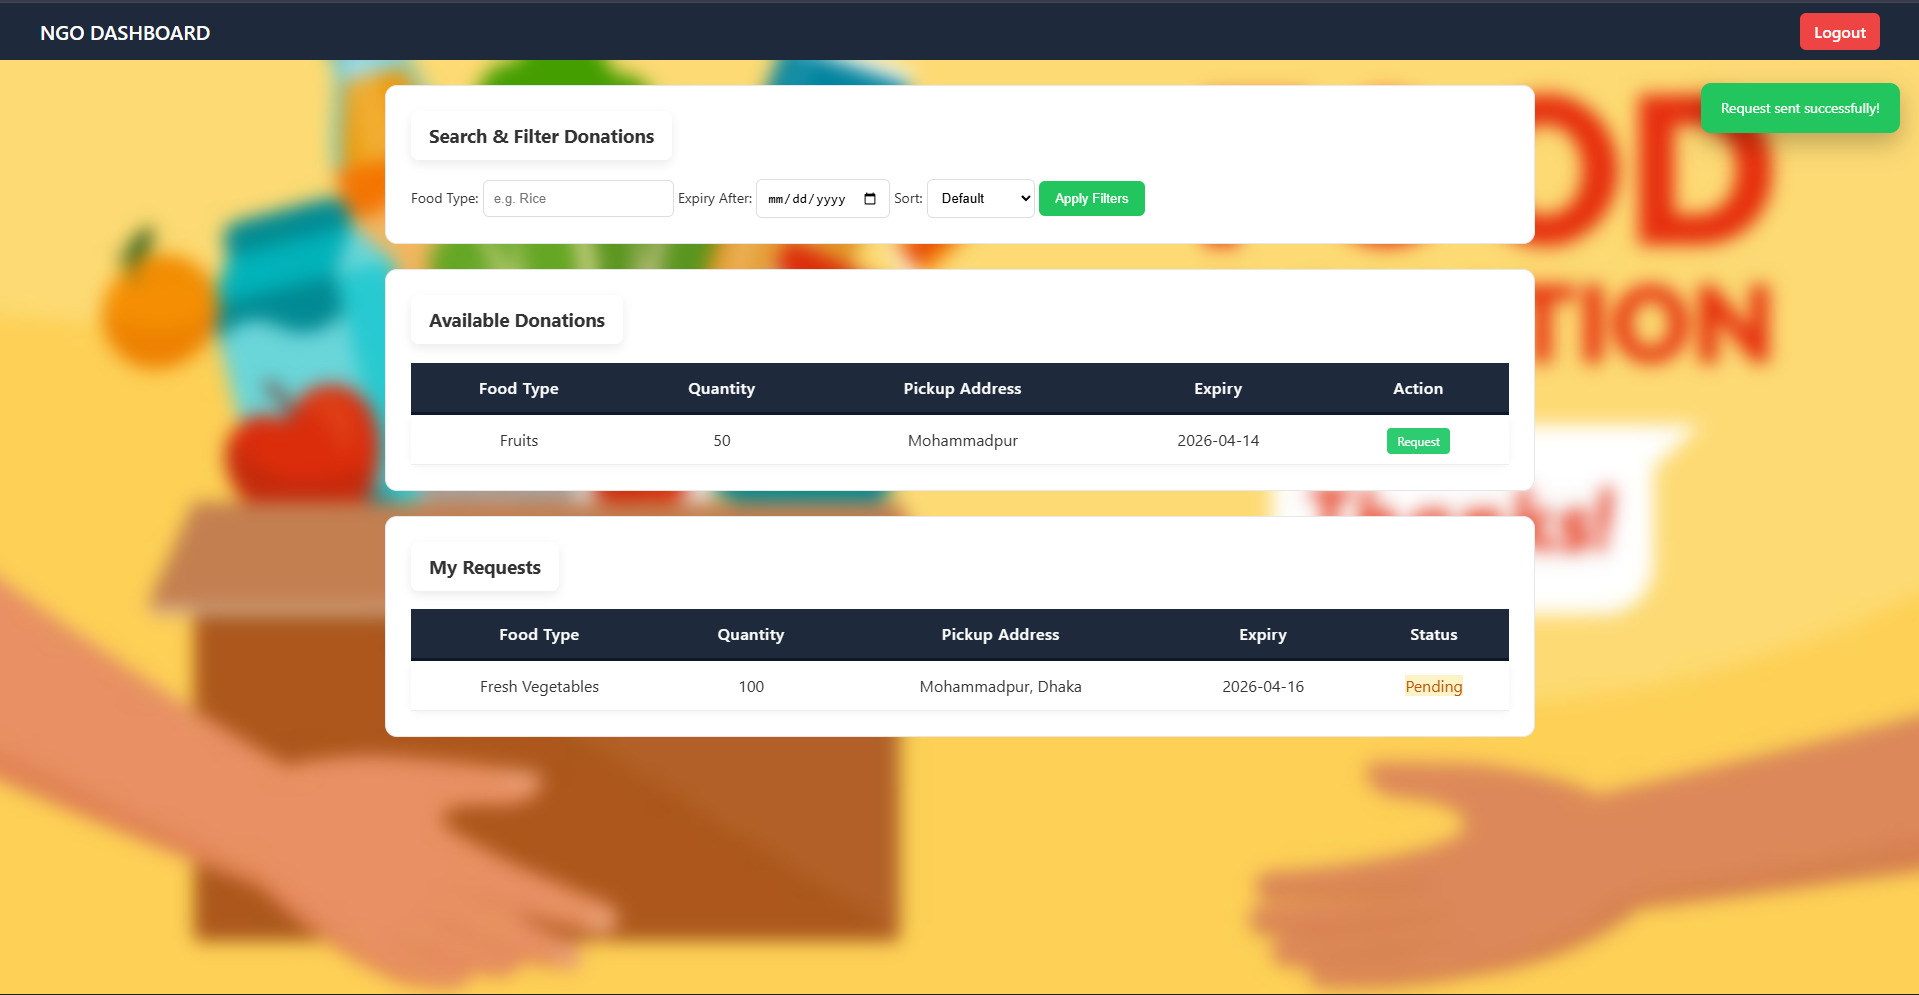
\includegraphics[width=0.90\textwidth]{Images/13. Donation Requested.jpg}

Donation Requested
\end{figure}
\FloatBarrier

\begin{figure}[h]
\centering
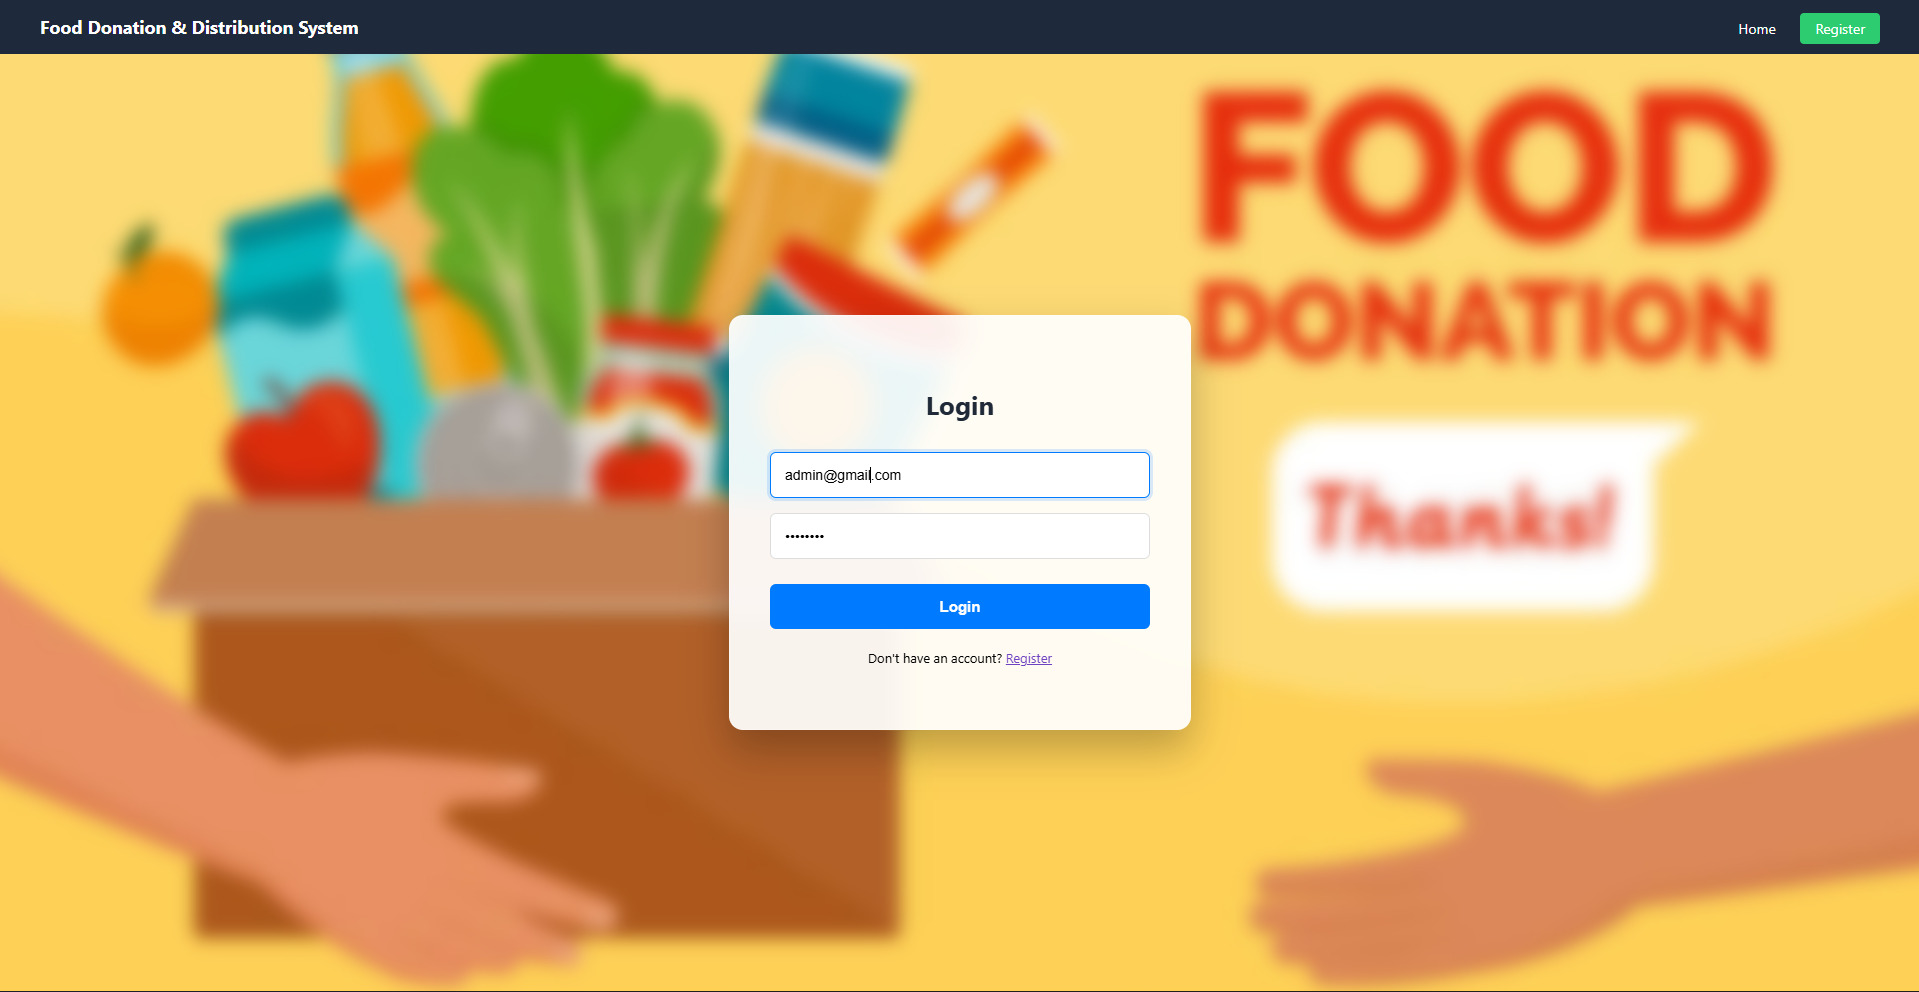
\includegraphics[width=0.90\textwidth]{Images/14. Login as Admin.jpg}

Login as Admin
\end{figure}
\FloatBarrier

\begin{figure}[h]
\centering
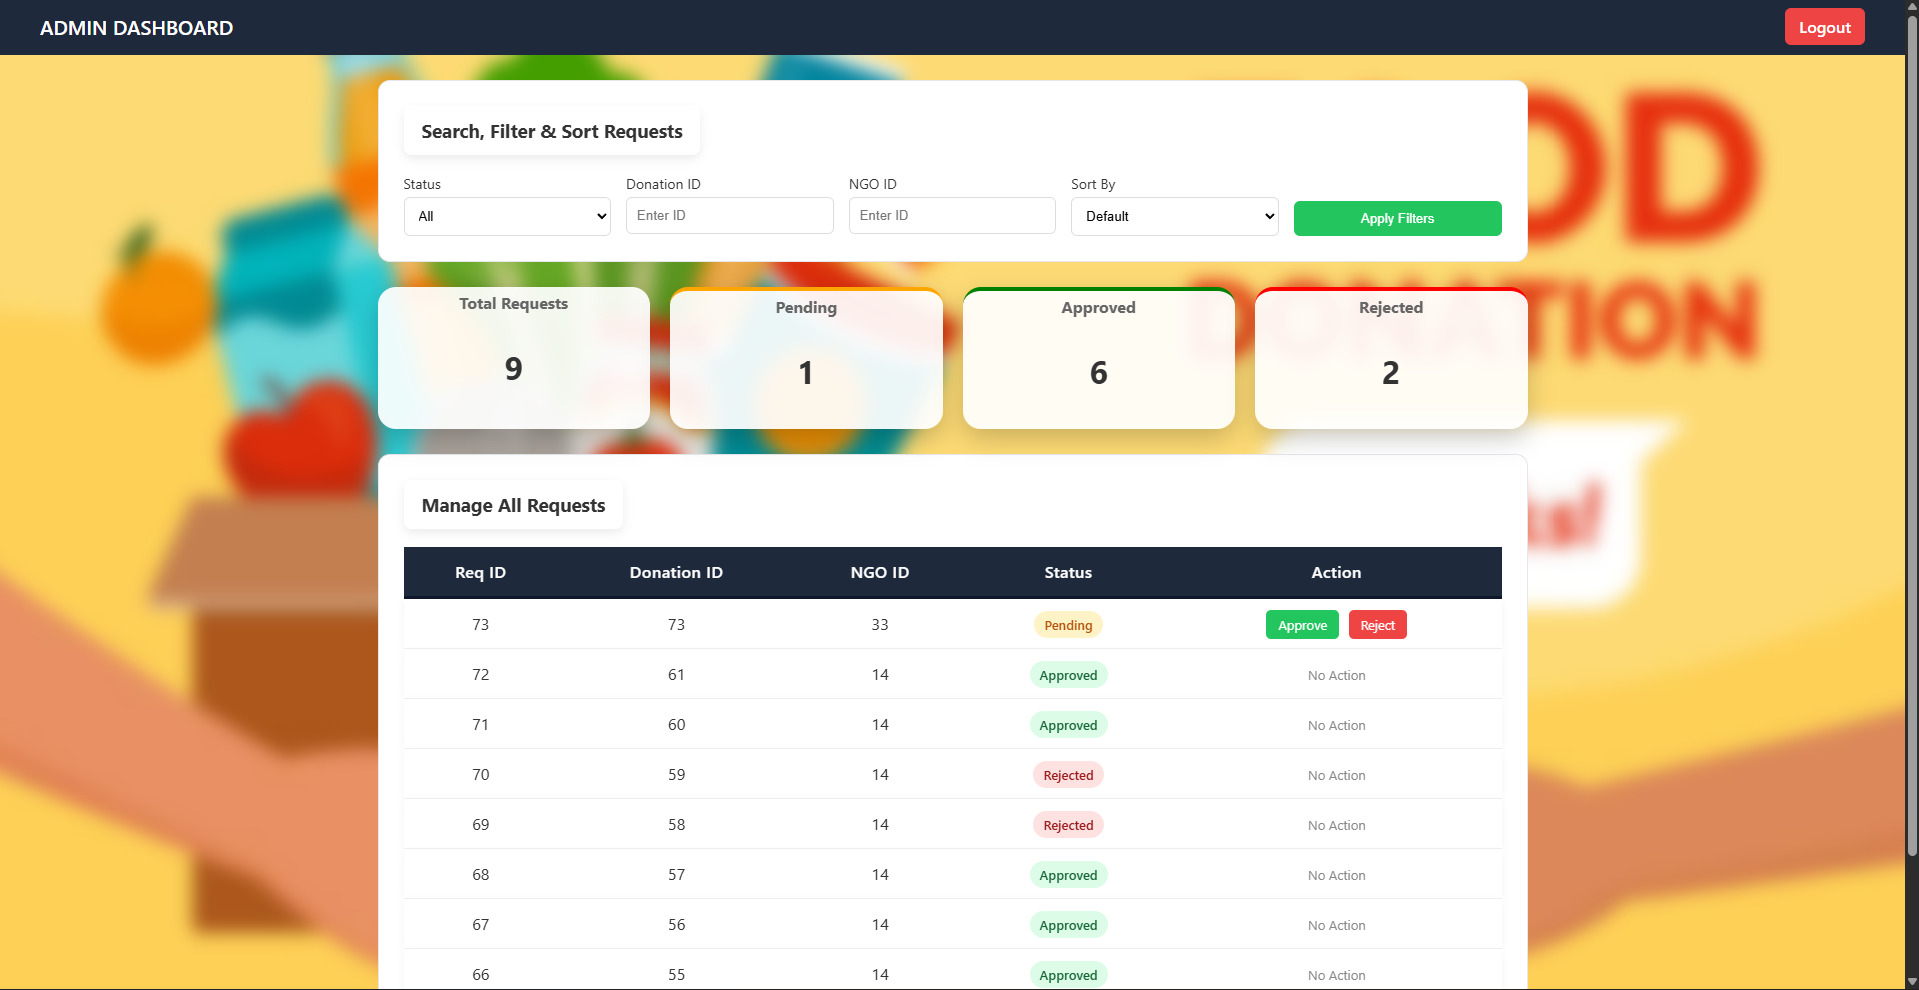
\includegraphics[width=0.90\textwidth]{Images/15. Admin Dashboard.jpg}

Admin Dashboard
\end{figure}
\FloatBarrier

\begin{figure}[h]
\centering
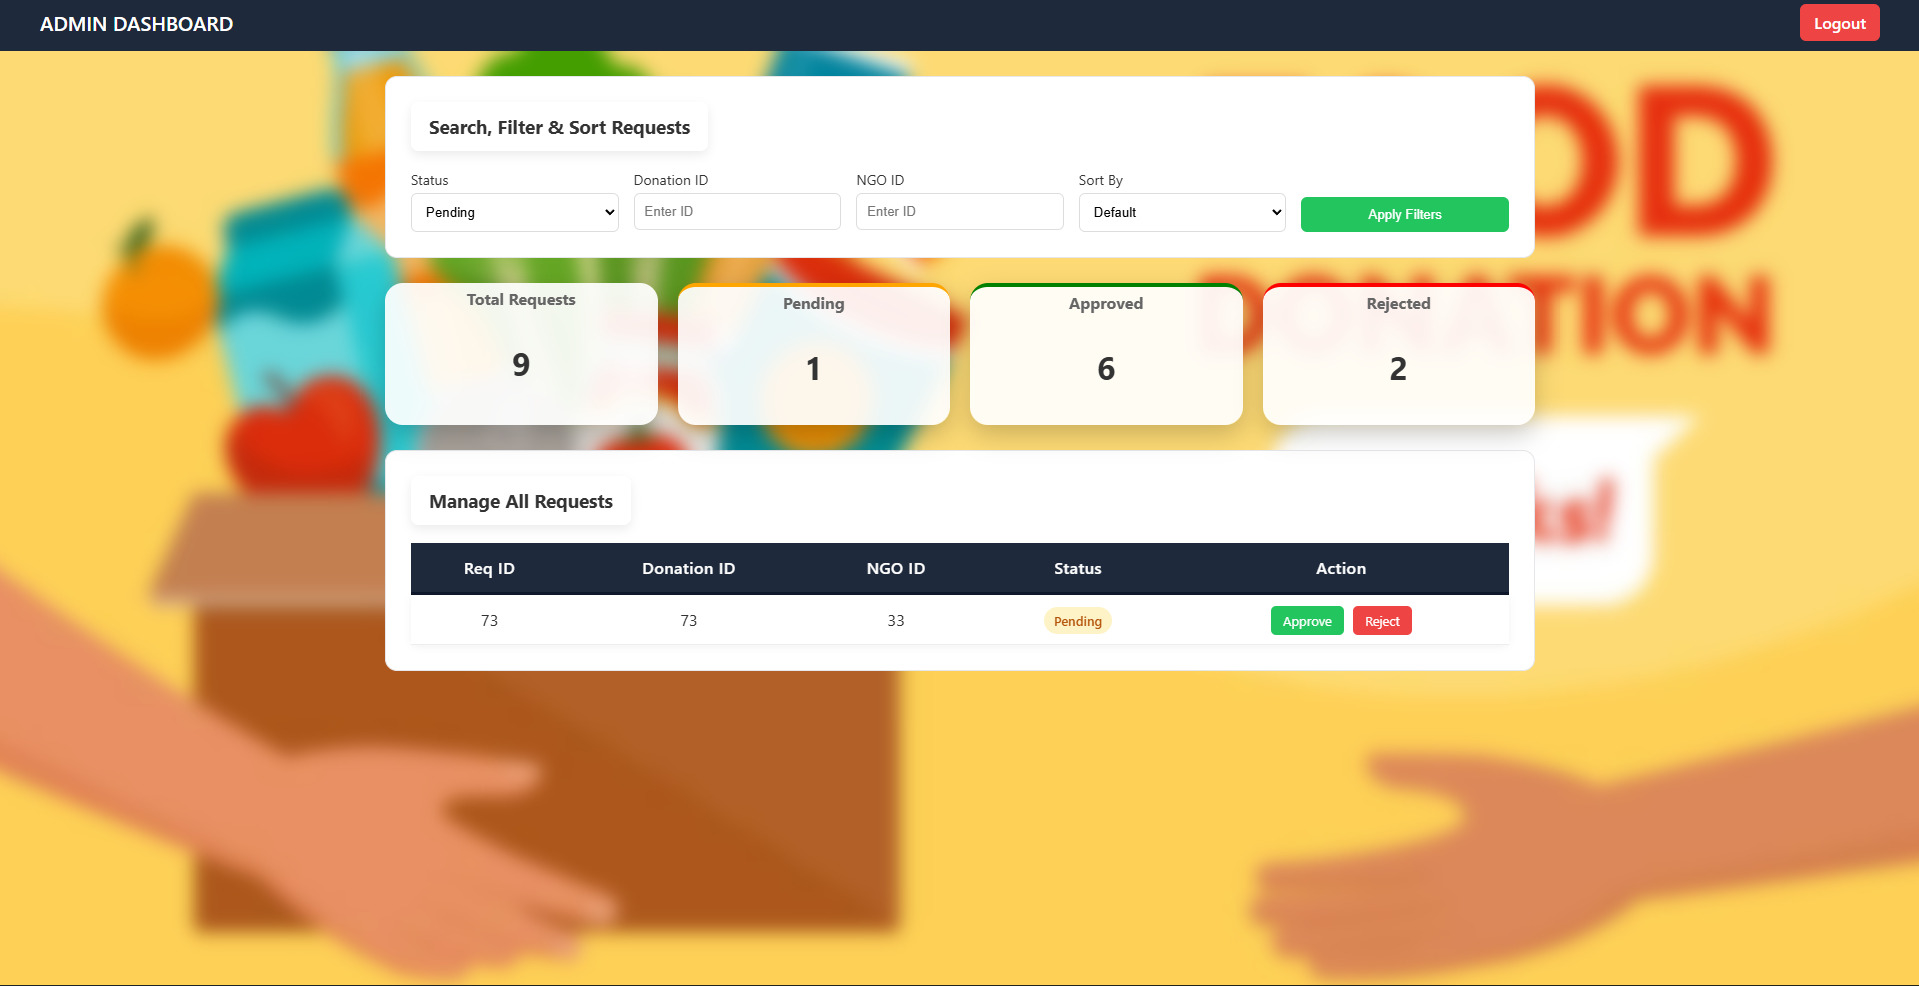
\includegraphics[width=0.90\textwidth]{Images/16. Sort Requests by 'Pending'.jpg}

Sort Requests by 'Pending'
\end{figure}
\FloatBarrier

\begin{figure}[h]
\centering
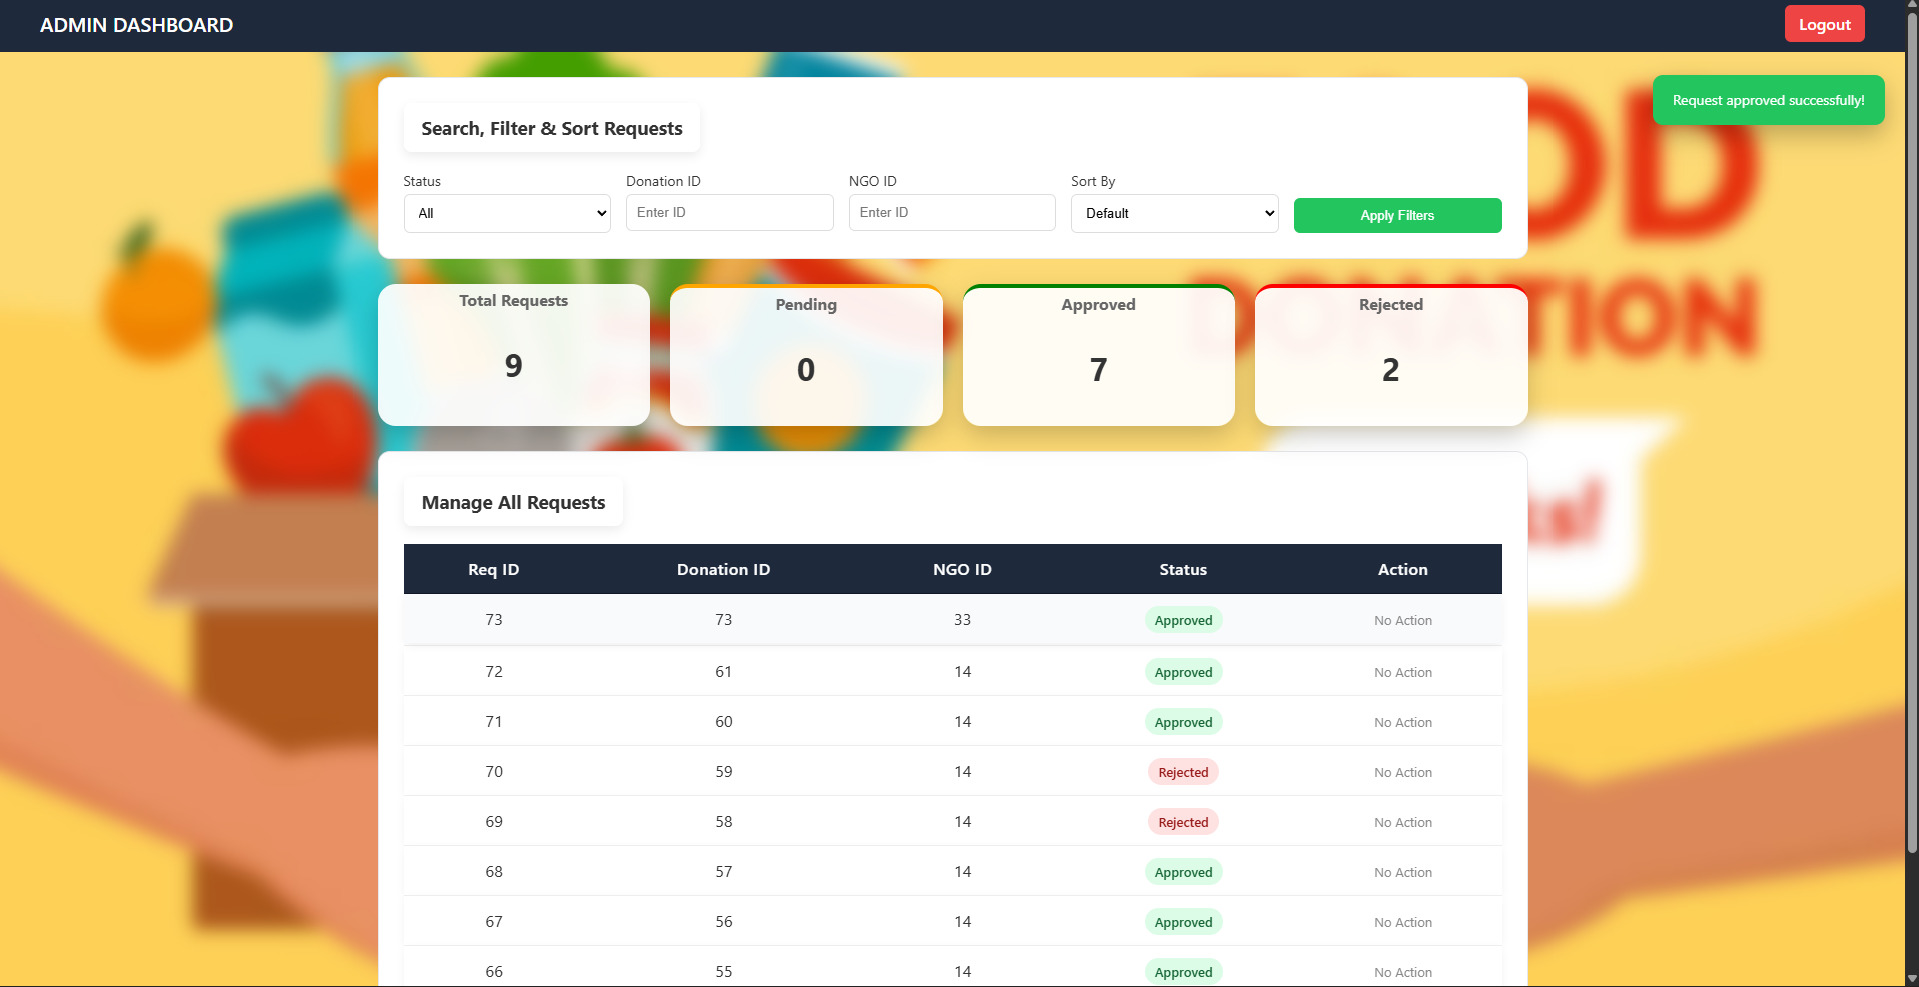
\includegraphics[width=0.90\textwidth]{Images/17. Request Approved.jpg}

Request Approved
\end{figure}
\FloatBarrier




\section{Conclusion}

The Food Donation Management System successfully provides a digital platform for connecting food donors with NGOs. The system helps reduce food waste and supports community welfare by facilitating efficient food distribution.

The platform demonstrates how technology can be used to solve social problems. With further development and deployment, the system could significantly improve food donation management and help address hunger in communities.






\vspace{200pt}
\section{Future Work and Limitations}

\textbf{Limitations}
\begin{itemize}
    \item No mobile application version
    \item No delivery tracking system
    \item Limited to web-based access
\end{itemize}

\vspace{60pt}
\textbf{Future Improvements}
\begin{itemize}
    \item Volunteer and Delivery service integration
    \item Mobile app integration
    \item GPS-based donation tracking
    \item Automated notification system
    \item Real-time chat between donors, NGOs and volunteers
    \item AI-based food demand prediction
\end{itemize}
